\newcounter{a}
\newcommand{\taskO}[1]{
	\refstepcounter{a}
	\label{#1}
}

\newcounter{b}[a]
\newcommand{\taskOO}[1]{
	\refstepcounter{b}
	\label{#1}
}

\section{Casi d'uso}
In questa sezione sono catalogati i casi d'uso derivati da un'attenta indagine ed analisi da parte dei membri del gruppo. Ognuno è identificato da un codice univoco e possiede una struttura interna accuratamente definita nel documento \NdP{}.
\subsection{Attori dei casi d'uso}
\textbf{Attori primari}
	\begin{itemize}
		\item \textbf{Utente non autenticato}: si riferisce all'utente del sistema che non ha ancora eseguito il login tramite \emph{Metamask}\ped{G};
		\item \textbf{Università}: si riferisce all'attore che ha effettuato il login tramite Metamask ed è stato autenticato e riconosciuto nel ruolo di \emph{Università};
		\item \textbf{Amministratore}: si riferisce all'attore che ha effettuato il login tramite Metamask ed è stato autenticato e riconosciuto nel ruolo di \emph\textbf{{Amministratore}}; possiede gli stessi privilegi di \emph{Università}, eccetto per la gestione dell'intera categoria di \emph{Amministratori};
		\item \textbf{Professore}: si riferisce all'attore che ha effettuato il login tramite Metamask ed è stato autenticato e riconosciuto nel ruolo di \emph{Professore};
		\item \textbf{Studente}: si riferisce all'attore che ha effettuato il login tramite Metamask ed è stato autenticato e riconosciuto nel ruolo di \emph{Studente}.
	\end{itemize}

\textbf{Attori secondari}
	\begin{itemize}
		\item \textbf{Metamask}: è un \emph{Ethereum Wallet}\ped{G} che permette di eseguire le DApp di Ethereum direttamente nel browser.
	\end{itemize}
\begin{figure} [H]
	\centering
	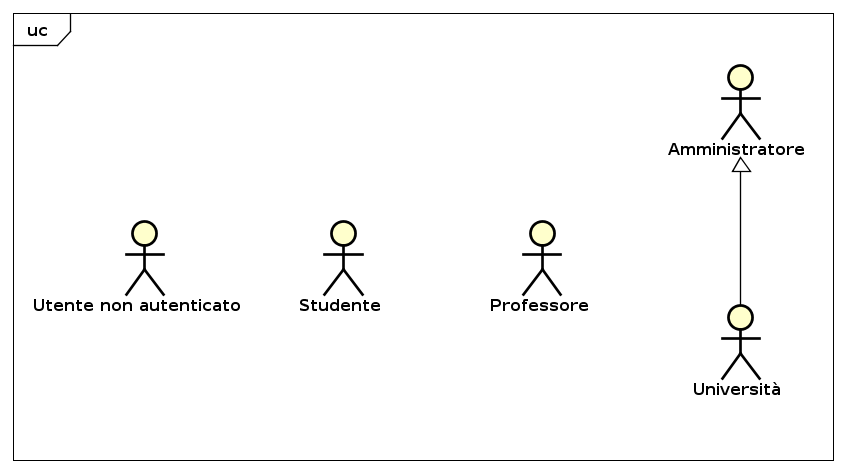
\includegraphics[scale=0.4]{./img/Attori.png}
	\caption{Gerarchia degli attori del sistema }\label{}
\end{figure}


%{UC0}{UC0}
\taskO{Scenario principale dell'utente non autenticato}
\subsection{Caso d'uso UC\ref{Scenario principale dell'utente non autenticato}: Scenario principale dell'utente non autenticato}
\begin{figure} [H]
	\centering
	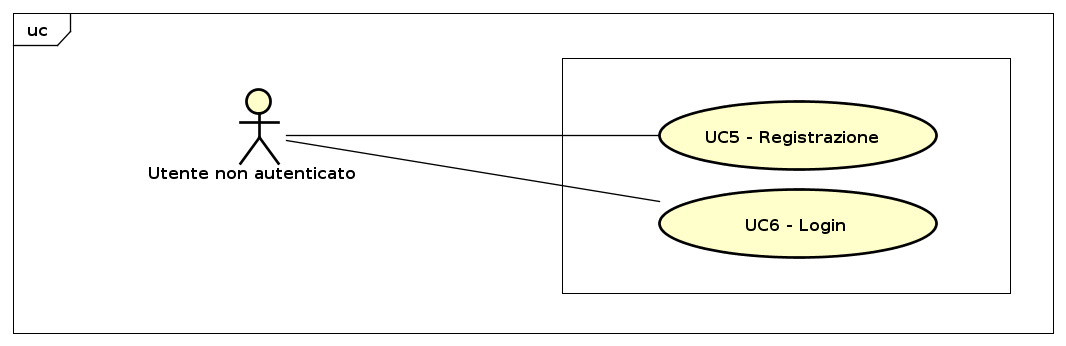
\includegraphics[scale=0.4]{./img/UseCaseDiagram01.png}
	\caption{Scenario principale }\label{}
\end{figure}
\begin{itemize}
	\item \textbf{Attori}: Utente non autenticato;
	\item \textbf{Descrizione}: Nella pagina principale un utente non autenticato può registrarsi se non possiede un account o se non ha un account Metamask valido, altrimenti viene autenticato automaticamente;
	\item \textbf{Precondizione}: Il sistema è avviato e mostra la pagina principale dell'applicazione;
	\item \textbf{Flusso principale degli eventi}: 
	\begin{itemize}
		\item Registrazione (UC\ref{Registrazione});
		\item Login (UC\ref{Login}).
	\end{itemize}
	\item \textbf{Postcondizione}: Il sistema ha ricevuto tutte le informazioni dall'utente non autenticato sulle operazioni che vuole eseguire.
\end{itemize}

\taskO{Scenario principale dell'universita e dell'amministratore}
\subsection{Caso d'uso UC\ref{Scenario principale dell'universita e dell'amministratore}: Scenario principale dell'università e dell'amministratore}
\begin{figure} [H]
	\centering
	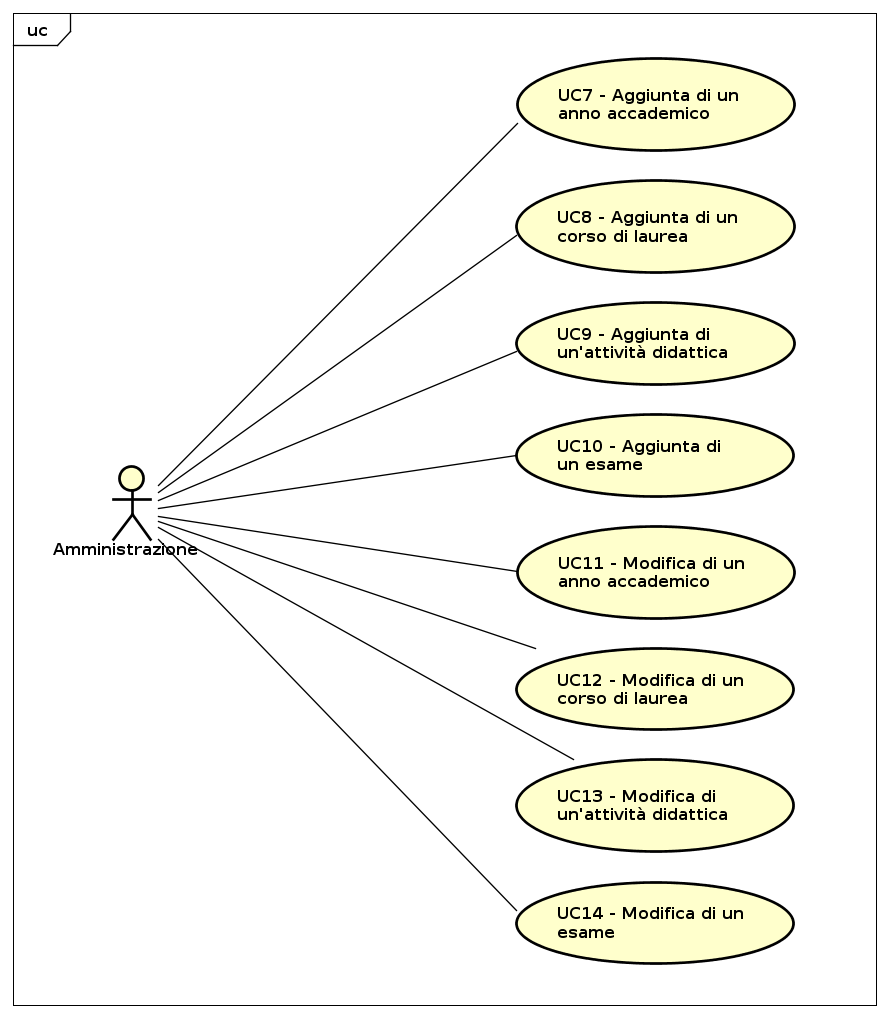
\includegraphics[scale=0.5]{./img/UseCaseDiagram02A.png}
	\caption{Scenario principale dell'amministrazione }\label{}
\end{figure}
	%\newpage
\begin{figure} [H]
	\centering
	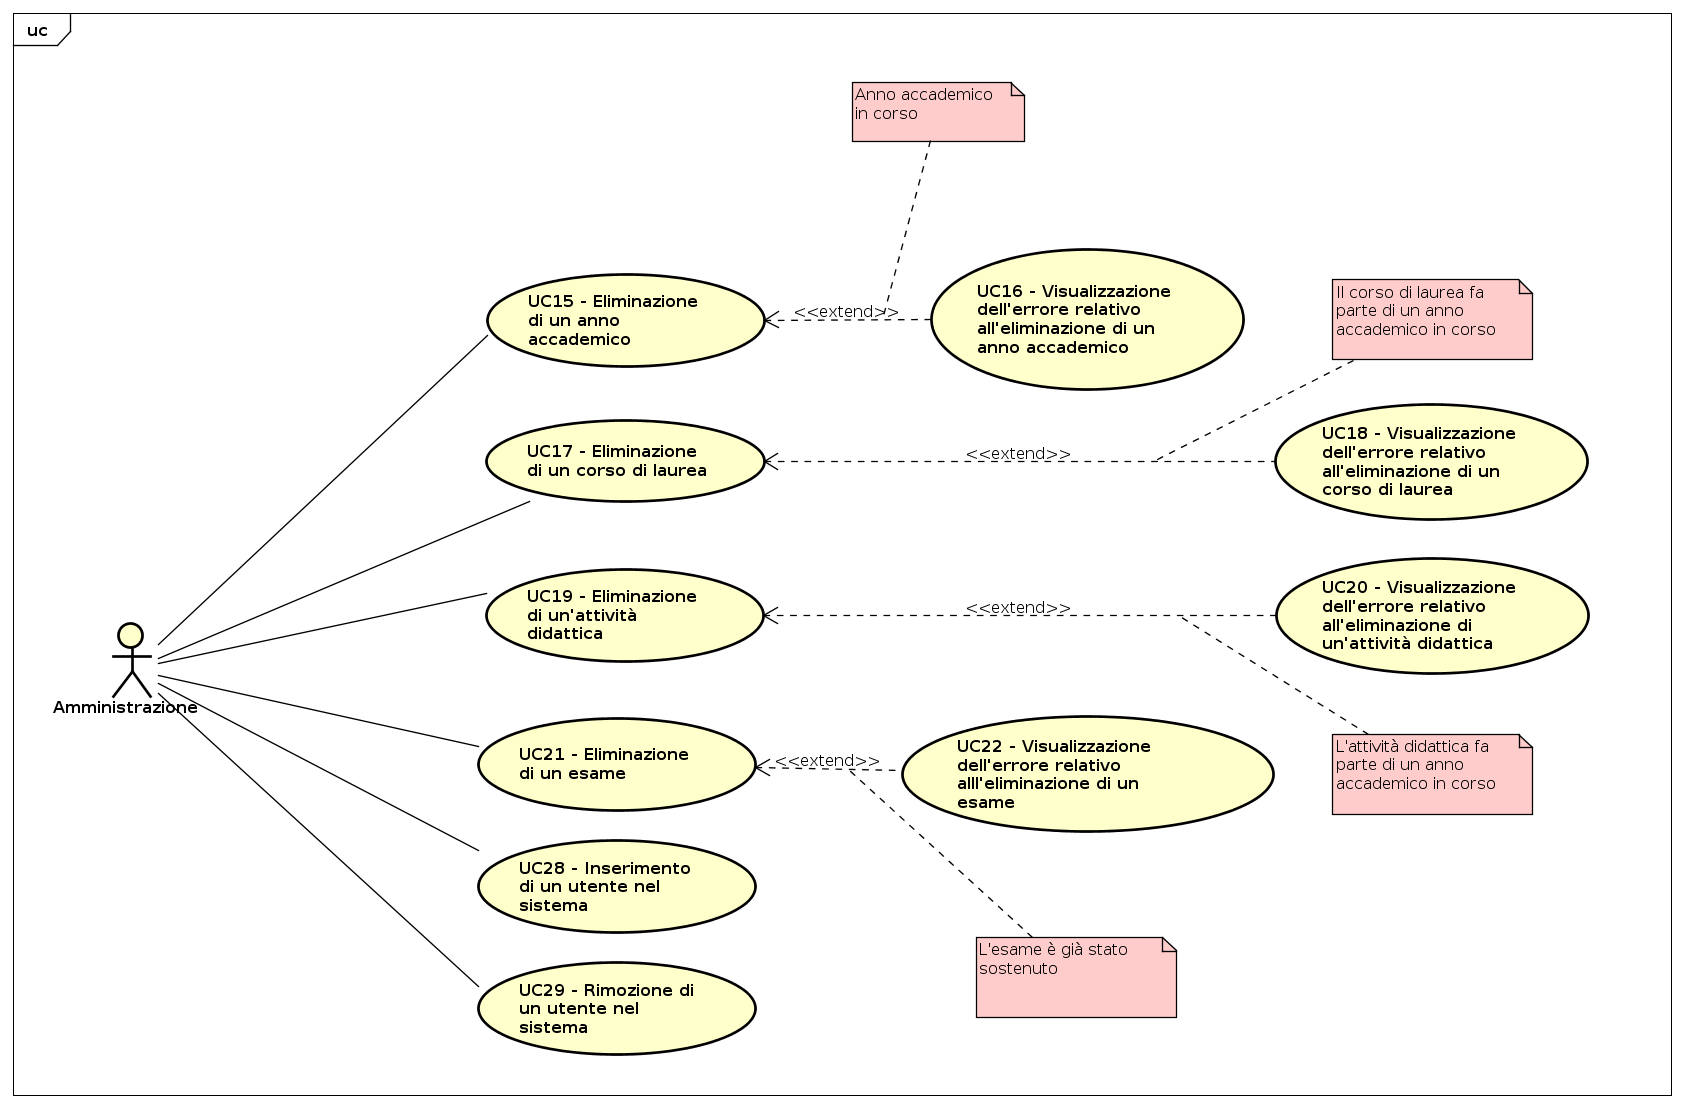
\includegraphics[scale=0.4]{./img/UseCaseDiagram02B.png}
	\caption{Scenario principale dell'amministrazione }\label{}
	\end{figure}
\begin{itemize}
	\item \textbf{Attori}: Università, Amministratore;
	\item \textbf{Descrizione}: L'università e l'amministratore possono: aggiungere, modificare, eliminare e visualizzare un errore di eliminazione relativo ad un anno accademico, un corso di laurea, un'attività didattica e un esame e possono inserire o rimuovere un utente dal sistema, mentre solo l'università può anche scegliere amministratore come tipologia di utente;
	\item \textbf{Precondizione}: Il sistema è avviato e mostra la pagina principale dell'applicazione;
	\item \textbf{Flusso principale degli eventi}: 
	\begin{itemize}
		\item Aggiunta di un anno accademico (UC\ref{Aggiunta di un anno accademico});
		\item Aggiunta di un corso di laurea (UC\ref{Aggiunta di un corso di laurea});
		\item Aggiunta di un'attivita didattica
		(UC\ref{Aggiunta di un'attivita didattica});
		\item Aggiunta di un esame
		(UC\ref{Aggiunta di un esame});
		\item Modifica di un anno accademico
		(UC\ref{Modifica di un anno accademico});
		\item Modifica di un corso di laurea
		(UC\ref{Modifica di un corso di laurea});
		\item Modifica di un'attività didattica
		(UC\ref{Modifica di un'attivita didattica});
		\item Modifica di un esame
		(UC\ref{Modifica di un esame});
		\item Eliminazione di un anno accademico
		(UC\ref{Eliminazione di un anno accademico});
		\item Visualizzazione dell’errore relativo all’eliminazione di un anno accademico 
		(UC\ref{Visualizzazione dell'errore relativo all'eliminazione di un anno accademico});
		\item Eliminazione di un corso di laurea
		(UC\ref{Eliminazione di un corso di laurea});
		\item Visualizzazione dell’errore relativo all’eliminazione di un corso di laurea
		(UC\ref{Visualizzazione dell'errore relativo all'eliminazione di un corso di laurea});
		\item Eliminazione di un'attività didattica
		(UC\ref{Eliminazione di un'attivita didattica});
		\item Visualizzazione dell’errore relativo all’eliminazione di un'attività didattica 
		(UC\ref{Visualizzazione dell'errore relativo all'eliminazione di un'attivita didattica});
		\item Eliminazione di un esame
		(UC\ref{Eliminazione di un esame});
		\item Visualizzazione dell’errore relativo all’eliminazione di un esame
		(UC\ref{Visualizzazione dell'errore relativo all'eliminazione di un esame});
		\item Inserimento di un utente nel sistema
		(UC\ref{Inserimento di un utente nel sistema});
		\item Inserimento della tipologia Amministratore
		(UC\ref{Inserimento della tipologia Amministratore});
		\item Rimozione di un utente dal sistema
		(UC\ref{Rimozione di un utente dal sistema}).
	\end{itemize}
	\item \textbf{Postcondizione}: Il sistema ha ricevuto tutte le informazioni dall'università o dall'amministratore sulle operazioni che vuole eseguire;
	\item \textbf{Estensioni}:
	\begin{itemize}
		\item Visualizzazione dell'errore relativo all'eliminazione di un anno accademico(UC13).
	\end{itemize}
\end{itemize}

\taskO{Scenario principale del professore}
\subsection{Caso d'uso UC\ref{Scenario principale del professore}: Scenario principale del professore}
\begin{figure} [H]
	\centering
	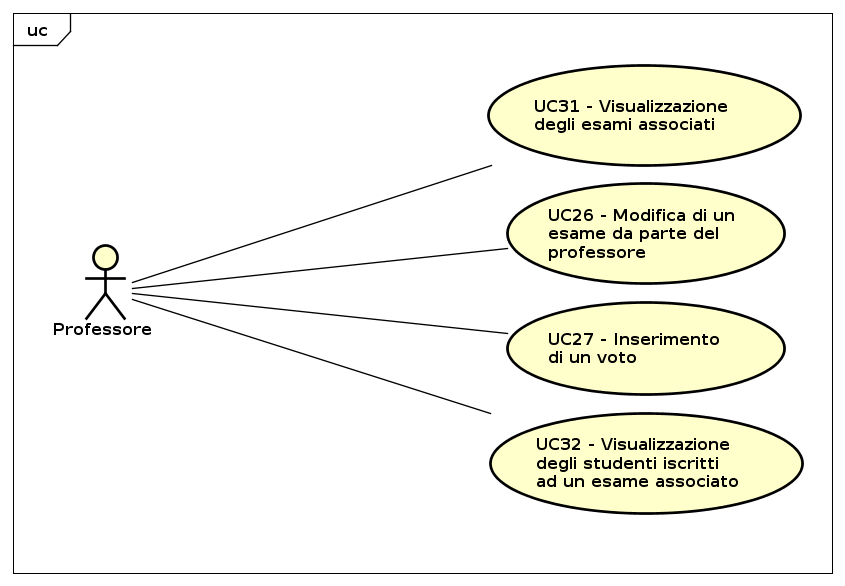
\includegraphics[scale=0.4]{./img/UseCaseDiagram03.png}
	\caption{Scenario principale }\label{}
\end{figure}
\begin{itemize}
	\item \textbf{Attori}: Professore;
	\item \textbf{Descrizione}: Un professore può vedere gli esami associati, modificare questi esami, inserire un voto e vedere gli studenti iscritti ai suoi esami;
	\item \textbf{Precondizione}: Il sistema è avviato e mostra la pagina principale dell'applicazione;
	\item \textbf{Flusso principale degli eventi}: 
	\begin{itemize}
		\item Modifica di un esame da parte di un professore
		(UC\ref{Modifica di un esame da parte di un professore});
		\item Inserimento di un voto
		(UC\ref{Inserimento di un voto});
		\item Visualizzazione degli esami associati
		(UC\ref{Visualizzazione degli esami associati});
		\item Visualizzazione degli studenti iscritti ad un esame associato
		(UC\ref{Visualizzazione degli studenti iscritti ad un esame associato}).
	\end{itemize}
	\item \textbf{Postcondizione}: Il sistema ha ricevuto tutte le informazioni dal professore sulle operazioni che vuole eseguire.
\end{itemize}

\taskO{Scenario principale dello studente}
\subsection{Caso d'uso UC\ref{Scenario principale dello studente}: Scenario principale dello studente}
\begin{figure} [H]
	\centering
	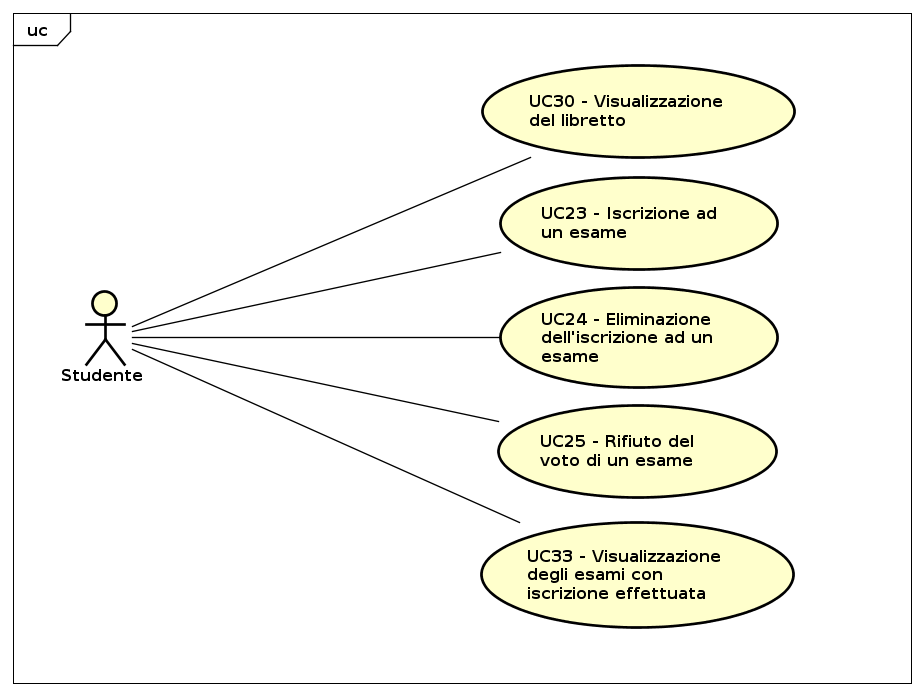
\includegraphics[scale=0.4]{./img/UseCaseDiagram04.png}
	\caption{Scenario principale }\label{}
\end{figure}
\begin{itemize}
	\item \textbf{Attori}: Studente;
	\item \textbf{Descrizione}: Uno studente può: vedere il proprio libretto, iscriversi ad un esame, eliminare l'iscrizione ad un esame e rifiutare un voto;
	\item \textbf{Precondizione}: Il sistema è avviato e mostra la pagina principale dell'applicazione;
	\item \textbf{Flusso principale degli eventi}: 
	\begin{itemize}
		\item Iscrizione ad un esame
		(UC\ref{Iscrizione ad un esame});
		\item Eliminazione dell’iscrizione ad un esame
		(UC\ref{Eliminazione dell'iscrizione ad un esame});
		\item Rifiuto del voto di un esame 
		(UC\ref{Rifiuto del voto di un esame});
		\item Visualizzazione del libretto
		(UC\ref{Visualizzazione del libretto})
		\item Visualizzazione degli esami con iscrizione effettuata
		(UC\ref{Visualizzazione degli esami con iscrizione effettuata}).
	\end{itemize}
	\item \textbf{Postcondizione}: Il sistema ha ricevuto tutte le informazioni dallo studente sulle operazioni che vuole eseguire.
\end{itemize}

\taskO{Registrazione}
\subsection{Caso d'uso UC\ref{Registrazione}: Registrazione }
\begin{figure} [H]
	\centering
	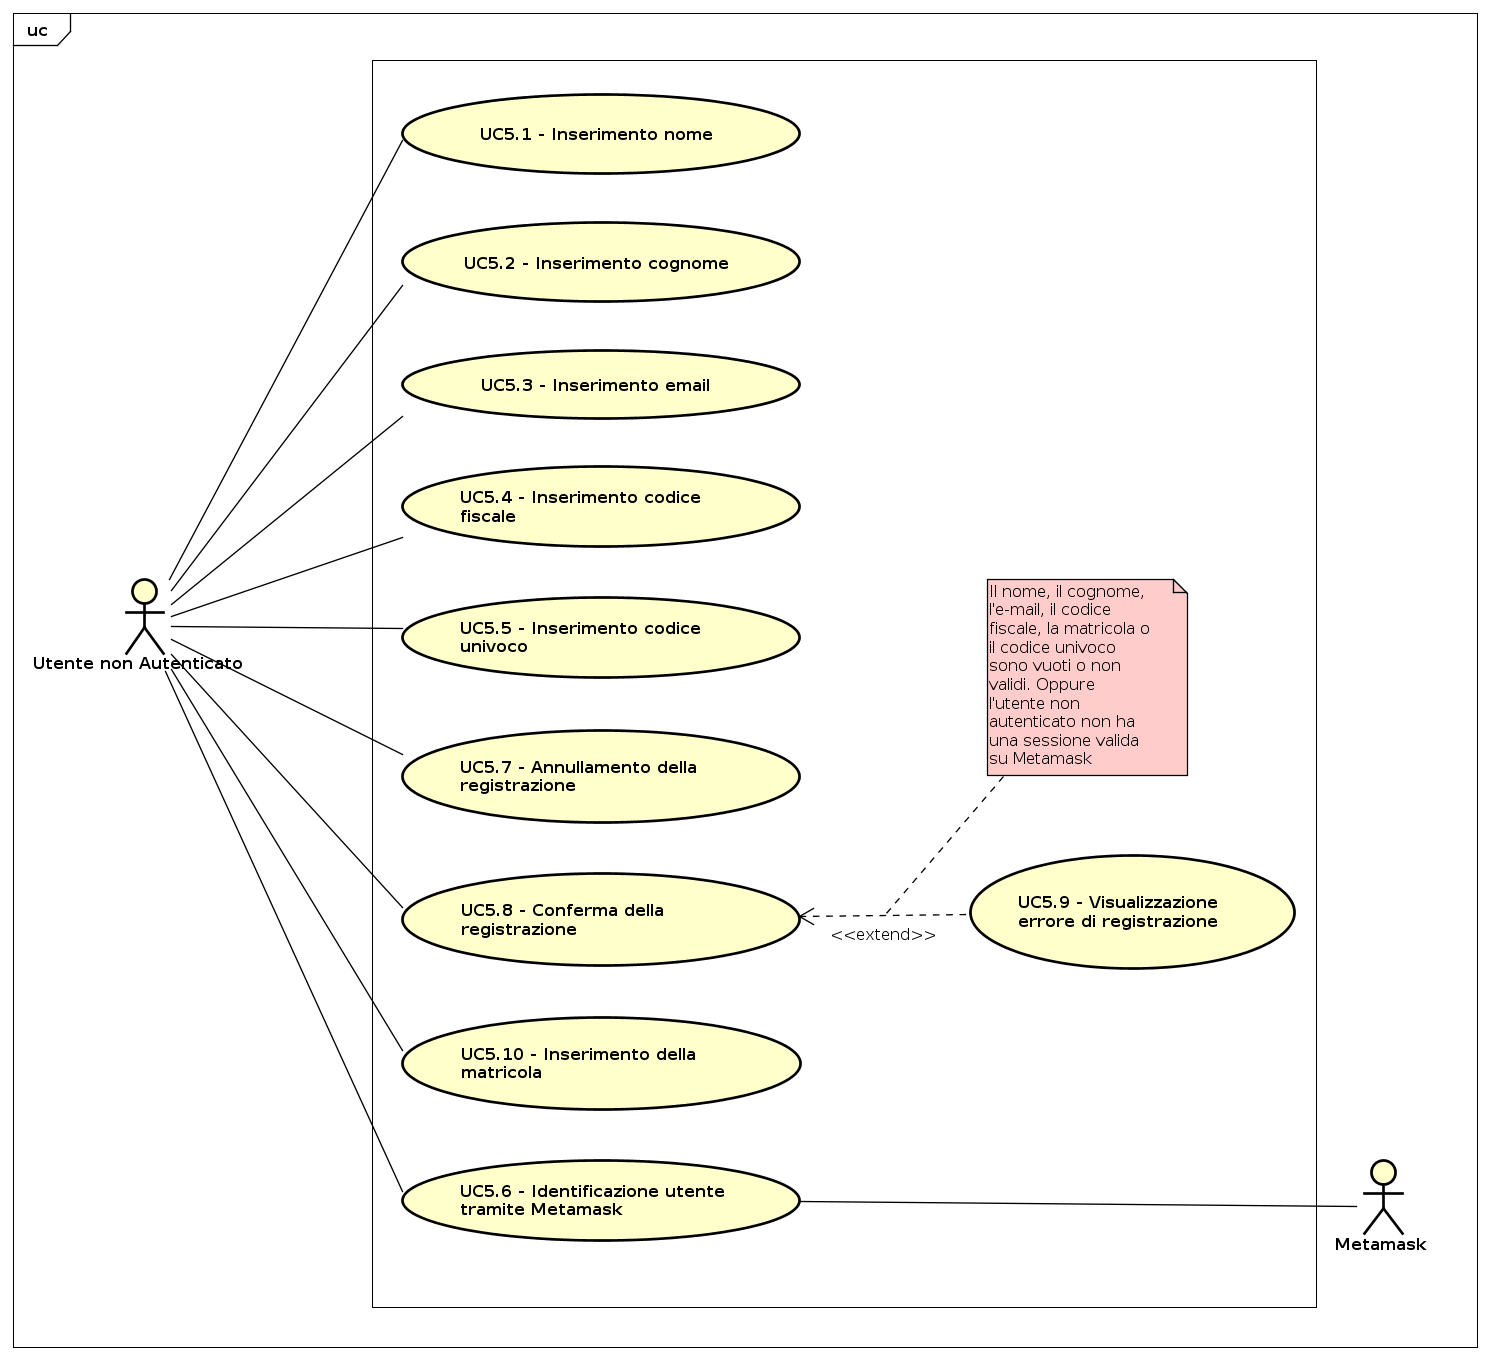
\includegraphics[scale=0.45]{./img/UseCaseDiagram05.png}
	\caption{Registrazione }\label{}
\end{figure}
\begin{itemize}
	\item \textbf{Attori}: Utente non autenticato, Metamask;
	\item \textbf{Descrizione}: Per accedere al sistema è necessario possedere un account;
	\item \textbf{Precondizione}: L'attore non possiede una account per accedere al sistema;
	\item \textbf{Flusso principale degli eventi}: L'attore si registra nel sistema attraverso i seguenti punti:
	\begin{itemize}
		\item Inserimento del nome (UC\ref{Registrazione}.\ref{Inserimento del nome});
		\item Inserimento del cognome (UC\ref{Registrazione}.\ref{Inserimento del cognome});
		\item Inserimento della e-mail (UC\ref{Registrazione}.\ref{Inserimento della e-mail});
		\item Inserimento del codice fiscale (UC\ref{Registrazione}.4);
		\item Inserimento del codice univoco (UC\ref{Registrazione}.5);
		\item Identificazione utente tramite Metamask (UC\ref{Registrazione}.6);
		\item Annullamento della registrazione (UC\ref{Registrazione}.7);
		\item Conferma della registrazione (UC\ref{Registrazione}.8);
		\item Visualizzazione dell'errore di registrazione (UC\ref{Registrazione}.9);
		\item Inserimento della matricola (UC\ref{Registrazione}.10).
	\end{itemize}
	\item \textbf{Postcondizione}: È stato creato un account per accedere al sistema.
\end{itemize}

\taskOO{Inserimento del nome}
\subsection{Caso d'uso UC\ref{Registrazione}.\ref{Inserimento del nome}: Inserimento del nome}
\begin{itemize}
	\item \textbf{Attori}: Utente non autenticato;
	\item \textbf{Descrizione}: L'attore deve inserire il proprio nome per potersi registrare;
	\item \textbf{Precondizione}: Il sistema fa visualizzare il campo di inserimento del nome;
	\item \textbf{Flusso principale degli eventi}: L'attore inserisce il proprio nome per effettuare la registrazione;
	\item \textbf{Postcondizione}: È stato inserito il nome dell'attore nel campo opportuno.
\end{itemize}

\taskOO{Inserimento del cognome}
\subsection{Caso d'uso UC\ref{Registrazione}.\ref{Inserimento del cognome}: Inserimento del cognome}
\begin{itemize}
	\item \textbf{Attori}: Utente non autenticato;
	\item \textbf{Descrizione}: L'attore deve inserire il proprio cognome per potersi registrare;
	\item \textbf{Precondizione}: Il sistema fa visualizzare il campo di inserimento del cognome;
	\item \textbf{Flusso principale degli eventi}: L'attore deve inserire il cognome per potersi registrare;
	\item \textbf{Postcondizione}: È stato inserito il cognome dell'attore nel campo opportuno.
\end{itemize}

\taskOO{Inserimento della e-mail}
\subsection{Caso d'uso UC\ref{Registrazione}.\ref{Inserimento della e-mail}: Inserimento della e-mail}
\begin{itemize}
	\item \textbf{Attori}: Utente non autenticato;
	\item \textbf{Descrizione}: L'attore deve inserire la proprio e-mail per potersi registrare;
	\item \textbf{Precondizione}: Il sistema fa visualizzare il campo di inserimento dell'e-mail;
	\item \textbf{Flusso principale degli eventi}: L'attore inserisce la propria e-mail per effettuare la registrazione;
	\item \textbf{Postcondizione}: È stata inserita la e-mail dell'attore nel campo opportuno.
\end{itemize}

\taskOO{Inserimento del codice fiscale}
\subsection{Caso d'uso UC\ref{Registrazione}.\ref{Inserimento del codice fiscale}: Inserimento del codice fiscale}
\begin{itemize}
	\item \textbf{Attori}: Utente non autenticato;
	\item \textbf{Descrizione}: L'attore deve inserire il proprio codice fiscale per potersi registrare;
	\item \textbf{Precondizione}: Il sistema fa visualizzare il campo di inserimento del codice fiscale;
	\item \textbf{Flusso principale degli eventi}: L'attore inserisce il proprio codice fiscale per effettuare la registrazione;
	\item \textbf{Postcondizione}: È stato inserito il codice fiscale dell'attore nel campo opportuno.
\end{itemize}

%{UC1.5}
\taskOO{Inserimento del codice univoco}
\subsection{Caso d'uso UC\ref{Registrazione}.\ref{Inserimento del codice univoco}: Inserimento del codice univoco}
\begin{itemize}
	\item \textbf{Attori}: Utente non autenticato;
	\item \textbf{Descrizione}: L'attore inserisce il codice univoco rilasciato dall'università per la registrazione;
	\item \textbf{Precondizione}: Il sistema fa visualizzare il campo di inserimento del codice univoco;
	\item \textbf{Flusso principale degli eventi}: L'attore inserisce il codice univoco per effettuare la registrazione;
	\item \textbf{Postcondizione}: È stato inserito il codice univoco dell'attore nel campo opportuno.
\end{itemize}

%{UC1.6}
\taskOO{Identificazione utente tramite Metamask}
\subsection{Caso d'uso UC\ref{Registrazione}.\ref{Identificazione utente tramite Metamask}: Identificazione utente tramite Metamask}
\begin{itemize}
	\item \textbf{Attori}: Utente non autenticato, Metamask;
	\item \textbf{Descrizione}: Il sistema sfrutta l'interfaccia Metamask per poter identificare univocamente l'utente;
	\item \textbf{Precondizione}: Il sistema fa visualizzare la pagina di registrazione utente;
	\item \textbf{Flusso principale degli eventi}: Il sistema ha bisogno dell'interfaccia Metamask per poter registrare un utente;
	\item \textbf{Postcondizione}: Il sistema ha identificato l'utente.
\end{itemize}

%{UC1.7}
\taskOO{Annullamento della registrazione}
\subsection{Caso d'uso UC\ref{Registrazione}.\ref{Annullamento della registrazione}: Annullamento della registrazione}
\begin{itemize}
	\item \textbf{Attori}: Utente non autenticato;
	\item \textbf{Descrizione}: L'attore decide di annullare la registrazione in corso;
	\item \textbf{Precondizione}: Il sistema fa visualizzare la pagina di registrazione;
	\item \textbf{Flusso principale degli eventi}: L'attore decide di annullare la registrazione, azione che aveva precedentemente intrapreso;
	\item \textbf{Postcondizione}: Il sistema non registra più l'attore in quanto esso ha annullato l'operazione.
\end{itemize}

%{UC1.8}
\taskOO{Conferma della registrazione}
\subsection{Caso d'uso UC\ref{Registrazione}.\ref{Conferma della registrazione}: Conferma della registrazione}
\begin{itemize}
	\item \textbf{Attori}: Utente non autenticato;
	\item \textbf{Descrizione}: L'attore può aver inserito tutti i dati  e conferma la registrazione;
	\item \textbf{Precondizione}: Il sistema fa visualizzare la pagina di registrazione;
	\item \textbf{Flusso principale degli eventi}: L'attore dopo aver inserito i dati può completare la registrazione confermandola;
	\item \textbf{Postcondizione}: Il sistema registra l'attore in quanto esso ha confermato la registrazione.
	\item \textbf{Estensioni}:
	\begin{itemize}
		\item Visualizzazione dell'errore di registrazione (UC1.9).
	\end{itemize}
\end{itemize}

%{UC1.9}
\taskOO{Visualizzazione dell'errore di registrazione}
\subsection{Caso d'uso UC\ref{Registrazione}.\ref{Visualizzazione dell'errore di registrazione}: Visualizzazione dell'errore di registrazione}
\begin{itemize}
	\item \textbf{Attori}: Utente non autenticato;
	\item \textbf{Descrizione}: L'attore può visualizzare un errore nel caso avesse inserito dati errati o non validi;
	\item \textbf{Precondizione}: Il sistema ha ricevuto campi dati errati, ovvero: già presenti, non validati o vuoti;
	\item \textbf{Flusso principale degli eventi}: L'attore visualizza un messaggio d'errore relativo all'inserimento mancato o non valido di:
	\begin{itemize}
		\item Nome;
		\item Cognome;
		\item E-mail (dove il sistema controlla che non sia già presente nel sistema);
		\item Codice fiscale; (dove il sistema controlla che non sia già presente nel sistema);
		\item Codice univoco;
		\item Metamask non attiva;
		\item Matricola.
	\end{itemize}
	\item \textbf{Postcondizione}: Il sistema fa visualizzare un messaggio d'errore riguardante il tentativo di registrazione con campi dati errati o vuoti.
\end{itemize}

%{UC1.10}
\taskOO{Inserimento della matricola}
\subsection{Caso d'uso UC\ref{Registrazione}.\ref{Inserimento della matricola}: Inserimento della matricola}
\begin{itemize}
	\item \textbf{Attori}: Utente non autenticato;
	\item \textbf{Descrizione}: L'attore inserisce la matricola ad esso associata dall'università per la registrazione;
	\item \textbf{Precondizione}: Il sistema fa visualizzare il campo di inserimento della matricola;
	\item \textbf{Flusso principale degli eventi}: L'attore inserisce la matricola per effettuare la registrazione;
	\item \textbf{Postcondizione}: È stata inserita la matricola dell'attore nel campo opportuno.
\end{itemize}

\taskO{Login}
\subsection{Caso d'uso UC\ref{Login}: Login}
%\begin{figure} [H]
%	\centering
%	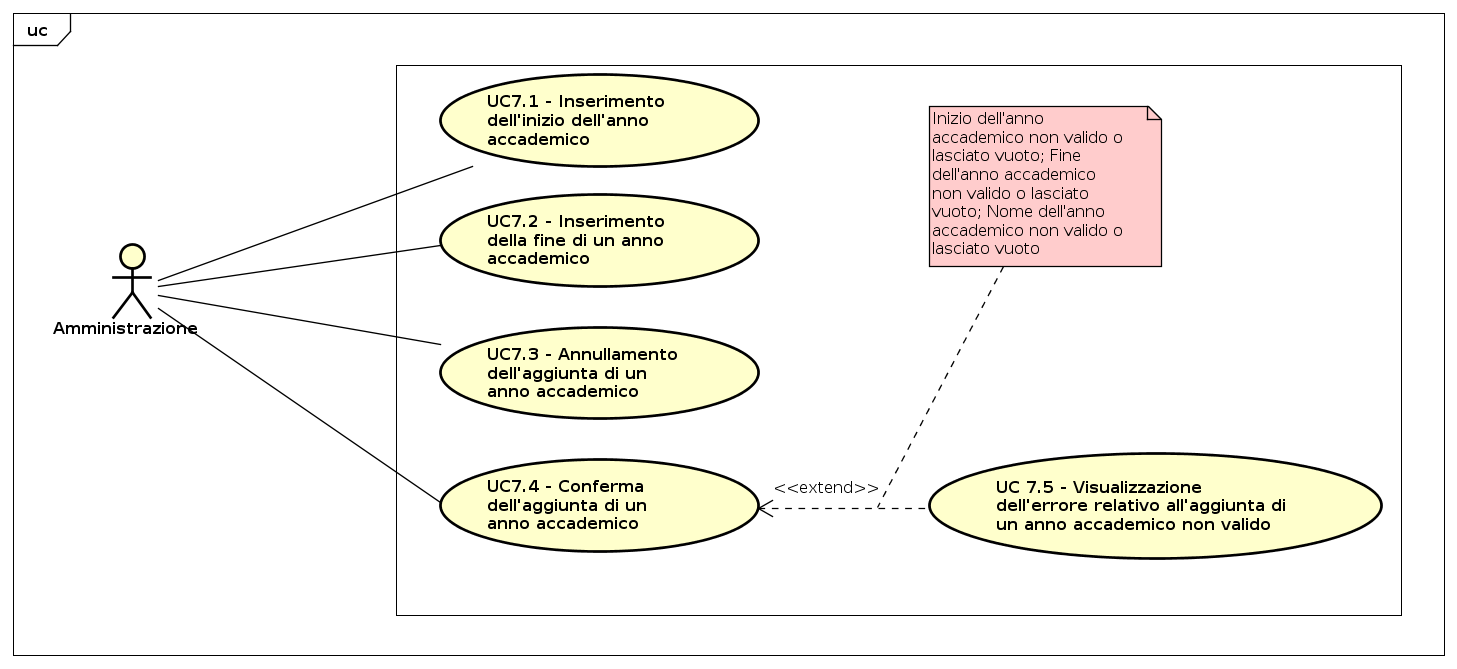
\includegraphics[scale=0.45]{./img/UseCaseDiagram07.png}
%	\caption{Login}\label{}
%\end{figure}
\begin{itemize}
	\item \textbf{Attori}: Utente non autenticato;
	\item \textbf{Descrizione}: Il sistema è avviato ma è necessario autenticarsi per accedervi;
	\item \textbf{Precondizione}: Il sistema non permette l'accesso all'attore non autenticato;
	\item \textbf{Flusso principale degli eventi}: L'attore effettua automaticamente il login;
	\item \textbf{Postcondizione}: Il sistema permette l'accesso all'attore che adesso è autenticato.
\end{itemize}

\taskO{Aggiunta di un anno accademico}
\subsection{Caso d'uso UC\ref{Aggiunta di un anno accademico}: Aggiunta di un anno accademico}
\begin{figure} [H]
	\centering
	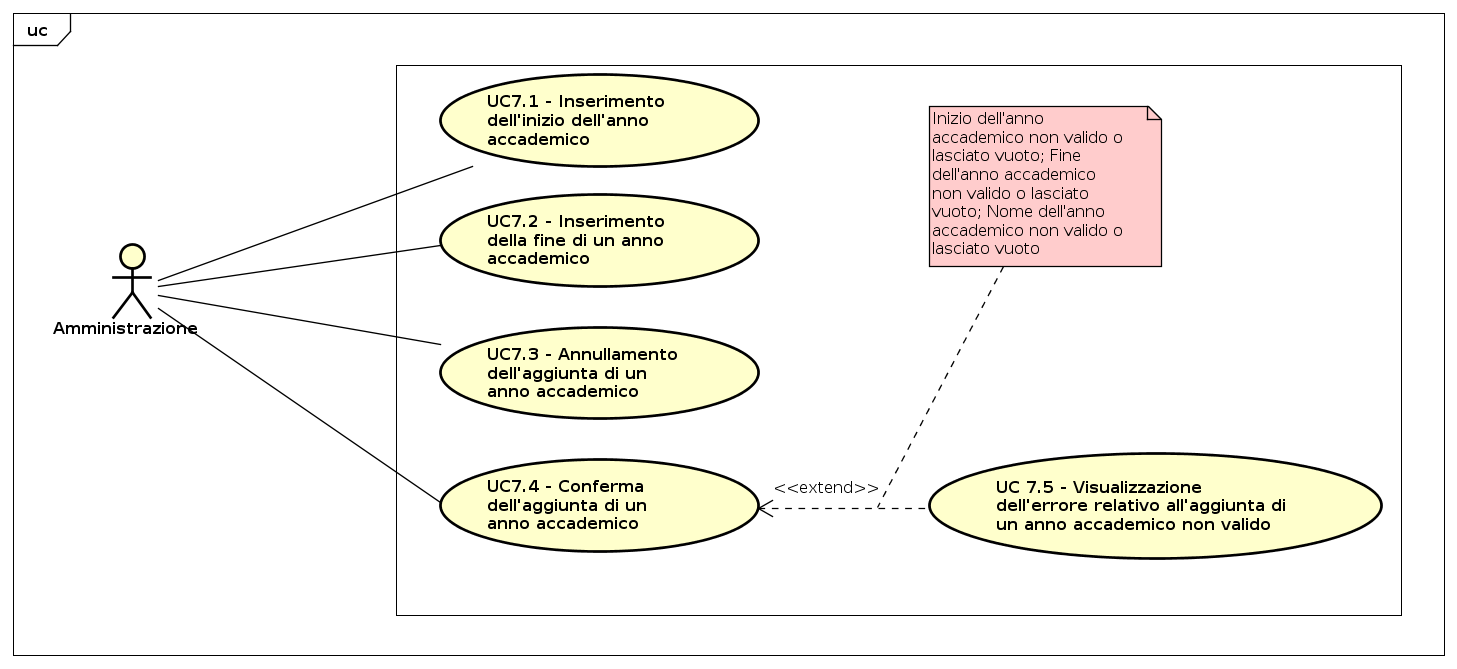
\includegraphics[scale=0.45]{./img/UseCaseDiagram07.png}
	\caption{Aggiunta di un anno accademico}\label{}
\end{figure}
\begin{itemize}
	\item \textbf{Attori}: Amministratore, Università;
	\item \textbf{Descrizione}: L'attore aggiunge un anno accademico alla lista degli anni accademici;
	\item \textbf{Precondizione}: La lista degli anni accademici è vuota oppure non contiene l'anno accademico che l'attore vuole inserire;
	\item \textbf{Flusso principale degli eventi}: L'attore, per inserire l'anno accademico alla lista, deve seguire i seguenti punti:
	\begin{itemize}
		\item Inserimento dell'inizio di un accademico (UC\ref{Aggiunta di un anno accademico}.\ref{Inserimento dell'inizio di un accademico});
		\item Inserimento della fine di un accademico (UC\ref{Aggiunta di un anno accademico}.\ref{Inserimento della fine di un accademico});
		\item Annullamento dell'aggiunta di un anno accademico (UC\ref{Aggiunta di un anno accademico}.\ref{Annullamento dell'aggiunta di un anno accademico});
		\item Conferma dell'aggiunta di un anno accademico (UC\ref{Aggiunta di un anno accademico}.\ref{Conferma dell'aggiunta di un anno accademico});
		\item Visualizzazione dell'errore relativo all'aggiunta di un anno accademico non valido (UC\ref{Aggiunta di un anno accademico}.\ref{Visualizzazione dell'errore relativo all'aggiunta di un anno accademico non valido});
		%\item Aggiunta di un corso di laurea (UC3.6).
	\end{itemize}
	\item \textbf{Postcondizione}: Il sistema può aver compilato dei campi relativi all'aggiunta di un nuovo anno accademico.
\end{itemize}

%{UC3.1}
\taskOO{Inserimento dell'inizio di un accademico}
\subsection{Caso d'uso UC\ref{Aggiunta di un anno accademico}.\ref{Inserimento dell'inizio di un accademico}: Inserimento dell'inizio di un accademico}
\begin{itemize}
	\item \textbf{Attori}: Amministratore, Università;
	\item \textbf{Descrizione}: L'attore compila il campo relativo all'inizio dell'anno accademico;
	\item \textbf{Precondizione}: Il sistema fa visualizzare il campo di inserimento dell'inizio dell'anno accademico;
	\item \textbf{Flusso principale degli eventi}: L'attore imposta l'inizio dell'anno accademico;
	\item \textbf{Postcondizione}: È stato inserito l'inizio dell'anno accademico nel campo opportuno.
\end{itemize}

%{UC3.2}
\taskOO{Inserimento della fine di un accademico}
\subsection{Caso d'uso UC\ref{Aggiunta di un anno accademico}.\ref{Inserimento della fine di un accademico}: Inserimento della fine di un accademico}
\begin{itemize}
	\item \textbf{Attori}: Amministratore, Università;
	\item \textbf{Descrizione}: L'attore compila il campo relativo alla fine dell'anno accademico;
	\item \textbf{Precondizione}: Il sistema fa visualizzare il campo di inserimento della fine dell'anno accademico;
	\item \textbf{Flusso principale degli eventi}: L'attore imposta la fine dell'anno accademico;
	\item \textbf{Postcondizione}: È stata inserita la fine dell'anno accademico nel campo opportuno.
\end{itemize}

%{UC3.3}:
\taskOO{Annullamento dell'aggiunta di un anno accademico}
\subsection{Caso d'uso UC\ref{Aggiunta di un anno accademico}.\ref{Annullamento dell'aggiunta di un anno accademico}: Annullamento dell'aggiunta di un anno accademico}
\begin{itemize}
	\item \textbf{Attori}: Amministratore, Università;
	\item \textbf{Descrizione}: L'attore può voler più aggiungere un anno accademico alla lista degli anni accademici;
	\item \textbf{Precondizione}: Il sistema fa visualizzare la pagina relativa all'aggiunta di un anno accademico;
	\item \textbf{Flusso principale degli eventi}: L'attore non inserisce più un anno accademico e quindi annulla l'operazione;
	\item \textbf{Postcondizione}: Il sistema non aggiunge più un anno accademico in quanto l'attore ha annullato l'operazione.
\end{itemize}

%{UC3.4}
\taskOO{Conferma dell'aggiunta di un anno accademico}
\subsection{Caso d'uso UC\ref{Aggiunta di un anno accademico}.\ref{Conferma dell'aggiunta di un anno accademico}: Conferma dell'aggiunta di un anno accademico}
\begin{itemize}
	\item \textbf{Attori}: Amministratore, Università;
	\item \textbf{Descrizione}: L'attore conferma l'aggiunta di un anno accademico alla lista degli anni accademici;
	\item \textbf{Precondizione}: Il sistema fa visualizzare la pagina relativa all'aggiunta di un anno accademico;
	\item \textbf{Flusso principale degli eventi}: L'attore, confermando l'inserimento dei dati, aggiunge un anno accademico alla lista degli anni accademici;
	\item \textbf{Postcondizione}: Il sistema aggiunge un anno accademico in quanto l'attore ha confermato l'operazione;
	\item \textbf{Estensioni}:
	\begin{itemize}
		\item Visualizzazione dell'errore relativo all'aggiunta di un anno accademico non valido (UC\ref{Aggiunta di un anno accademico}.\ref{Visualizzazione dell'errore relativo all'aggiunta di un anno accademico non valido}).
	\end{itemize}
\end{itemize}

%{UC3.5}
\taskOO{Visualizzazione dell'errore relativo all'aggiunta di un anno accademico non valido}
\subsection{Caso d'uso UC\ref{Aggiunta di un anno accademico}.\ref{Visualizzazione dell'errore relativo all'aggiunta di un anno accademico non valido}: Visualizzazione dell'errore relativo all'aggiunta di un anno accademico non valido}
\begin{itemize}
	\item \textbf{Attori}: Amministratore, Università;
	\item \textbf{Descrizione}: L'attore aggiunge i dettagli di un anno accademico senza rispettarne la validazione;
	\item \textbf{Precondizione}: Il sistema ha ricevuto campi dati errati o vuoti;
	\item \textbf{Flusso principale degli eventi}: L'attore, impostando in maniera errata i campi dell'anno accademico, può visualizzare uno dei seguenti errori:
	\begin{itemize}
		\item Inizio dell'anno accademico non valido o lasciato vuoto;
		\item Fine dell'anno accademico non valido o lasciato vuoto;
		\item Nome dell'anno accademico non valido o lasciato vuoto.
	\end{itemize}
	\item \textbf{Postcondizione}: Il sistema fa visualizzare un messaggio d'errore riguardante il tentativo di aggiungere un anno accademico con campi dati errati o vuoti.
\end{itemize}







%{UC3.6}
\taskO{Aggiunta di un corso di laurea}
\subsection{Caso d'uso UC\ref{Aggiunta di un corso di laurea}: Aggiunta di un corso di laurea}
\begin{figure} [H]
	\centering
	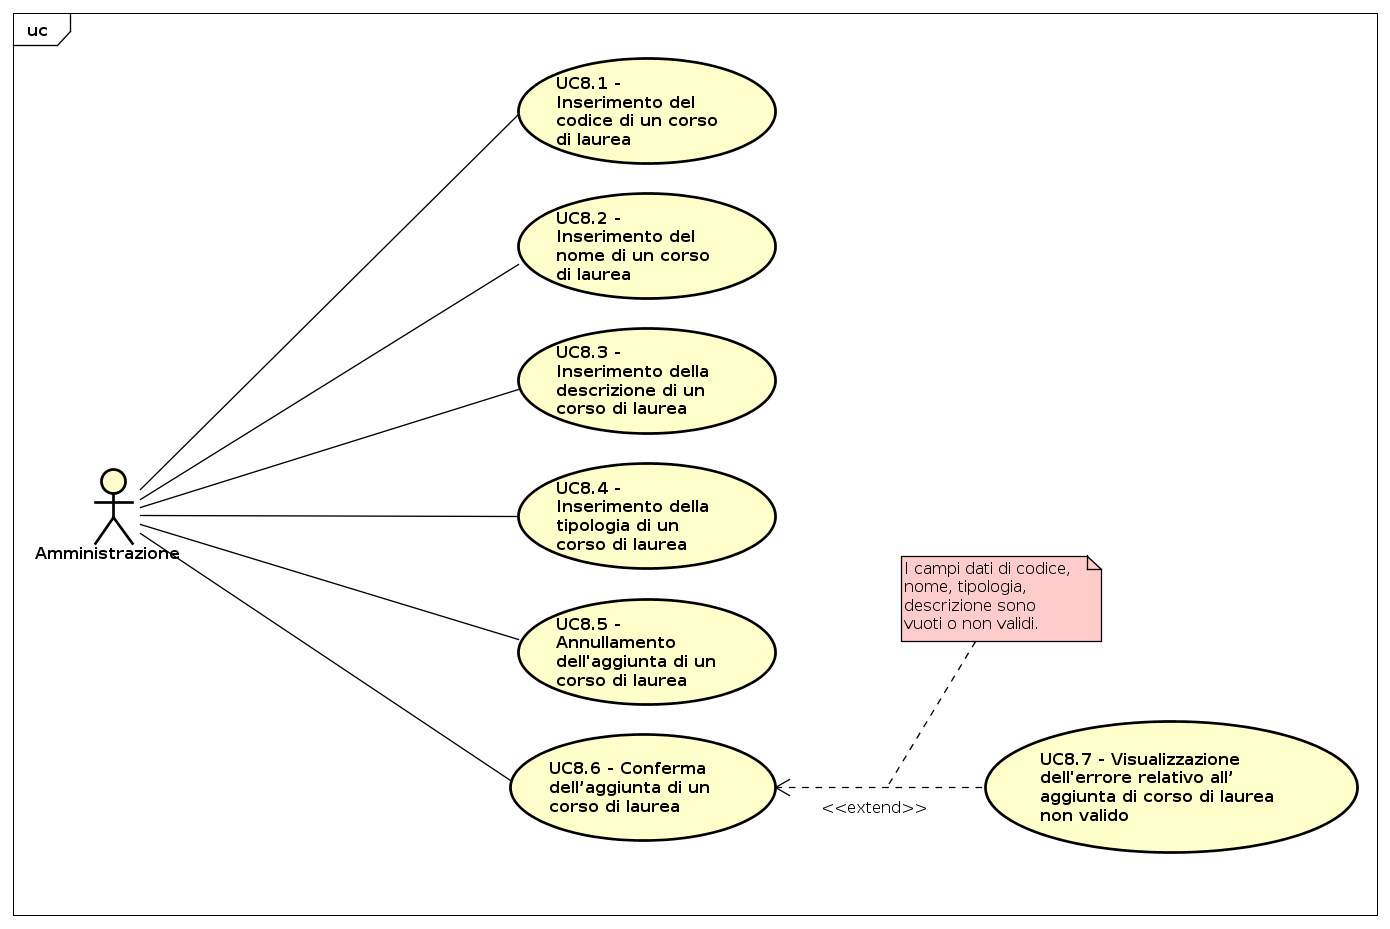
\includegraphics[scale=0.45]{./img/UseCaseDiagram08.png}
	\caption{Aggiunta di un corso di laurea}\label{}
\end{figure}
\begin{itemize}
	\item \textbf{Attori}: Amministratore, Università;
	\item \textbf{Descrizione}: L'attore aggiunge un corso di laurea alla lista dei corsi di laurea;
	\item \textbf{Precondizione}: La lista dei corsi di laurea è vuota oppure non contiene il corso di laurea che l'attore vuole inserire;
	\item \textbf{Flusso principale degli eventi}: L'attore, per inserire il corso di laurea alla lista, deve seguire i seguenti punti:
	\begin{itemize}
		\item Inserimento del codice di un corso di laurea (UC\ref{Aggiunta di un corso di laurea}.\ref{Inserimento del codice di un corso di laurea});
		\item Inserimento del nome di un corso di laurea (UC\ref{Aggiunta di un corso di laurea}.\ref{Inserimento del nome di un corso di laurea});
		\item Inserimento della descrizione di un corso di laurea (UC\ref{Aggiunta di un corso di laurea}.\ref{Inserimento della descrizione di un corso di laurea});
		\item Inserimento della tipologia di un corso di laurea (UC\ref{Aggiunta di un corso di laurea}.\ref{Inserimento della tipologia di un corso di laurea});
		\item Annullamento dell'aggiunta di un corso di laurea (UC\ref{Aggiunta di un corso di laurea}.\ref{Annullamento dell'aggiunta di un corso di laurea});
		\item Conferma dell'aggiunta di un corso di laurea (UC\ref{Aggiunta di un corso di laurea}.\ref{Conferma dell'aggiunta di un corso di laurea});
		%\item Aggiunta di un'attività didattica (UC3.6.7);
		\item Visualizzazione dell'errore relativo all'aggiunta di corso di laurea non valido (UC\ref{Aggiunta di un corso di laurea}.\ref{Visualizzazione dell'errore relativo all'aggiunta di corso di laurea non valido}).
	\end{itemize}
	\item \textbf{Postcondizione}: Il sistema può aver compilato dei campi relativi all'aggiunta di un nuovo corso di laurea.
\end{itemize}





%{UC3.6.1}
\taskOO{Inserimento del codice di un corso di laurea}
\subsection{Caso d'uso UC\ref{Aggiunta di un corso di laurea}.\ref{Inserimento del codice di un corso di laurea}: Inserimento del codice di un corso di laurea}
\begin{itemize}
	\item \textbf{Attori}: Amministratore, Università;
	\item \textbf{Descrizione}: L'attore compila il campo relativo al codice del corso di laurea;
	\item \textbf{Precondizione}: Il sistema fa visualizzare il campo di inserimento del codice di un corso di laurea;
	\item \textbf{Flusso principale degli eventi}: L'attore imposta il codice del corso di laurea;
	\item \textbf{Postcondizione}: È stato inserito il codice del corso di laurea nel campo opportuno.
\end{itemize}



%{UC3.6.2}
\taskOO{Inserimento del nome di un corso di laurea}
\subsection{Caso d'uso UC\ref{Aggiunta di un corso di laurea}.\ref{Inserimento del nome di un corso di laurea}: Inserimento del nome di un corso di laurea}
\begin{itemize}
	\item \textbf{Attori}: Amministratore, Università;
	\item \textbf{Descrizione}: L'attore compila il campo relativo al nome del corso di laurea;
	\item \textbf{Precondizione}: Il sistema fa visualizzare il campo di inserimento del nome di un corso di laurea;
	\item \textbf{Flusso principale degli eventi}: L'attore imposta il nome del corso di laurea;
	\item \textbf{Postcondizione}: È stato inserito il nome del corso di laurea nel campo opportuno.
\end{itemize}

%{UC3.6.3}
\taskOO{Inserimento della descrizione di un corso di laurea}
\subsection{Caso d'uso UC\ref{Aggiunta di un corso di laurea}.\ref{Inserimento della descrizione di un corso di laurea}: Inserimento della descrizione di un corso di laurea}
\begin{itemize}
	\item \textbf{Attori}: Amministratore, Università;
	\item \textbf{Descrizione}: L'attore compila il campo relativo alla descrizione del corso di laurea;
	\item \textbf{Precondizione}: Il sistema fa visualizzare il campo di inserimento della descrizione di un corso di laurea;
	
	\item \textbf{Flusso principale degli eventi}: L'attore aggiunge la descrizione del corso di laurea;
	\item \textbf{Postcondizione}: È stata inserita la descrizione del corso di laurea nel campo opportuno.
\end{itemize}

%{UC3.6.4}
\taskOO{Inserimento della tipologia di un corso di laurea}
\subsection{Caso d'uso UC\ref{Aggiunta di un corso di laurea}.\ref{Inserimento della tipologia di un corso di laurea}: Inserimento della tipologia di un corso di laurea}
\begin{itemize}
	\item \textbf{Attori}: Amministratore, Università;
	\item \textbf{Descrizione}: L'attore compila il campo relativo alla tipologia del corso di laurea;
	\item \textbf{Precondizione}: Il sistema fa visualizzare il campo di inserimento della tipologia di un corso di laurea;
	\item \textbf{Flusso principale degli eventi}: L'attore aggiunge la tipologia del corso di laurea, scegliendo fra:
		\begin{itemize}
			\item Triennale;
			\item Magistrale;
			\item Ciclo unico;
		\end{itemize}
	\item \textbf{Postcondizione}: È stata inserita la tipologia del corso di laurea nel campo opportuno.
\end{itemize}

%{UC3.6.5}
\taskOO{Annullamento dell'aggiunta di un corso di laurea}
\subsection{Caso d'uso UC\ref{Aggiunta di un corso di laurea}.\ref{Annullamento dell'aggiunta di un corso di laurea}: Annullamento dell'aggiunta di un corso di laurea}
\begin{itemize}
	\item \textbf{Attori}: Amministratore, Università;
	\item \textbf{Descrizione}: L'attore non aggiunge più un corso di laurea alla lista dei corsi di laurea;
	
	\item \textbf{Precondizione}: l sistema fa visualizzare la pagina relativa all'aggiunta di un corso di laurea;
	
	\item \textbf{Flusso principale degli eventi}: L'attore non inserisce più un corso di laurea e quindi annulla l'operazione;
	
	\item \textbf{Postcondizione}: Il sistema non aggiunge più un corso di laurea in quanto l'attore ha annullato l'operazione.
	
\end{itemize}

%{UC3.6.6}
\taskOO{Conferma dell'aggiunta di un corso di laurea}
\subsection{Caso d'uso UC\ref{Aggiunta di un corso di laurea}.\ref{Conferma dell'aggiunta di un corso di laurea}: Conferma dell'aggiunta di un corso di laurea}
\begin{itemize}
	\item \textbf{Attori}: Amministratore, Università;
	\item \textbf{Descrizione}: L'attore conferma l'aggiunta di corso di laurea alla lista dei corsi di laurea;
	
	\item \textbf{Precondizione}: Il sistema fa visualizzare la pagina relativa all'aggiunta di un corso di laurea;
	
	\item \textbf{Flusso principale degli eventi}: L'attore, confermando l'inserimento dei dati, aggiunge un corso di laurea alla lista dei corsi di laurea;
	
	\item \textbf{Postcondizione}: Il sistema aggiunge un corso di laurea in quanto l'attore ha confermato l'operazione;
	
	\item \textbf{Estensioni}:
	\begin{itemize}
		\item Visualizzazione dell'errore relativo all'aggiunta di corso di laurea non valido (UC\ref{Aggiunta di un corso di laurea}.\ref{Visualizzazione dell'errore relativo all'aggiunta di corso di laurea non valido}).
	\end{itemize}
\end{itemize}

%{UC3.6.8}
\taskOO{Visualizzazione dell'errore relativo all'aggiunta di corso di laurea non valido}
\subsection{Caso d'uso UC\ref{Aggiunta di un corso di laurea}.\ref{Visualizzazione dell'errore relativo all'aggiunta di corso di laurea non valido}: Visualizzazione dell'errore relativo all'aggiunta di corso di laurea non valido }
\begin{itemize}
	\item \textbf{Attori}: Amministratore, Università;
	\item \textbf{Descrizione}: L'attore aggiunge i dettagli di un corso di laurea senza rispettarne la validazione;
	
	\item \textbf{Precondizione}: Il sistema ha ricevuto campi dati errati o vuoti;
	
	\item \textbf{Flusso principale degli eventi}: L'attore, impostando in maniera errata i campi del corso di laurea, può visualizzare uno dei seguenti errori: 
	\begin{itemize}
		\item Codice del corso di laurea non valido o lasciato vuoto;
		\item Nome del corso di laurea non valido o lasciato vuoto;
		\item Descrizione del corso di laurea non valido o lasciato vuoto;
		\item Codice del corso di laurea non valido o lasciato vuoto;
		\item Tipologia del corso di laurea non valido o lasciato vuoto;
		\item Codice dell'anno accademico non valido o lasciato vuoto;
		\item Attività didattica del corso di laurea non valida o lasciata vuota.
	\end{itemize}
	
	\item \textbf{Postcondizione}: Il sistema fa visualizzare un messaggio d'errore riguardante il tentativo di aggiungere un corso di laurea con campi dati errati o vuoti.
	
\end{itemize}





%{UC3.6.7}
\taskO{Aggiunta di un'attivita didattica}
\subsection{Caso d'uso UC\ref{Aggiunta di un'attivita didattica}: Aggiunta di un'attività didattica}
\begin{figure} [H]
	\centering
	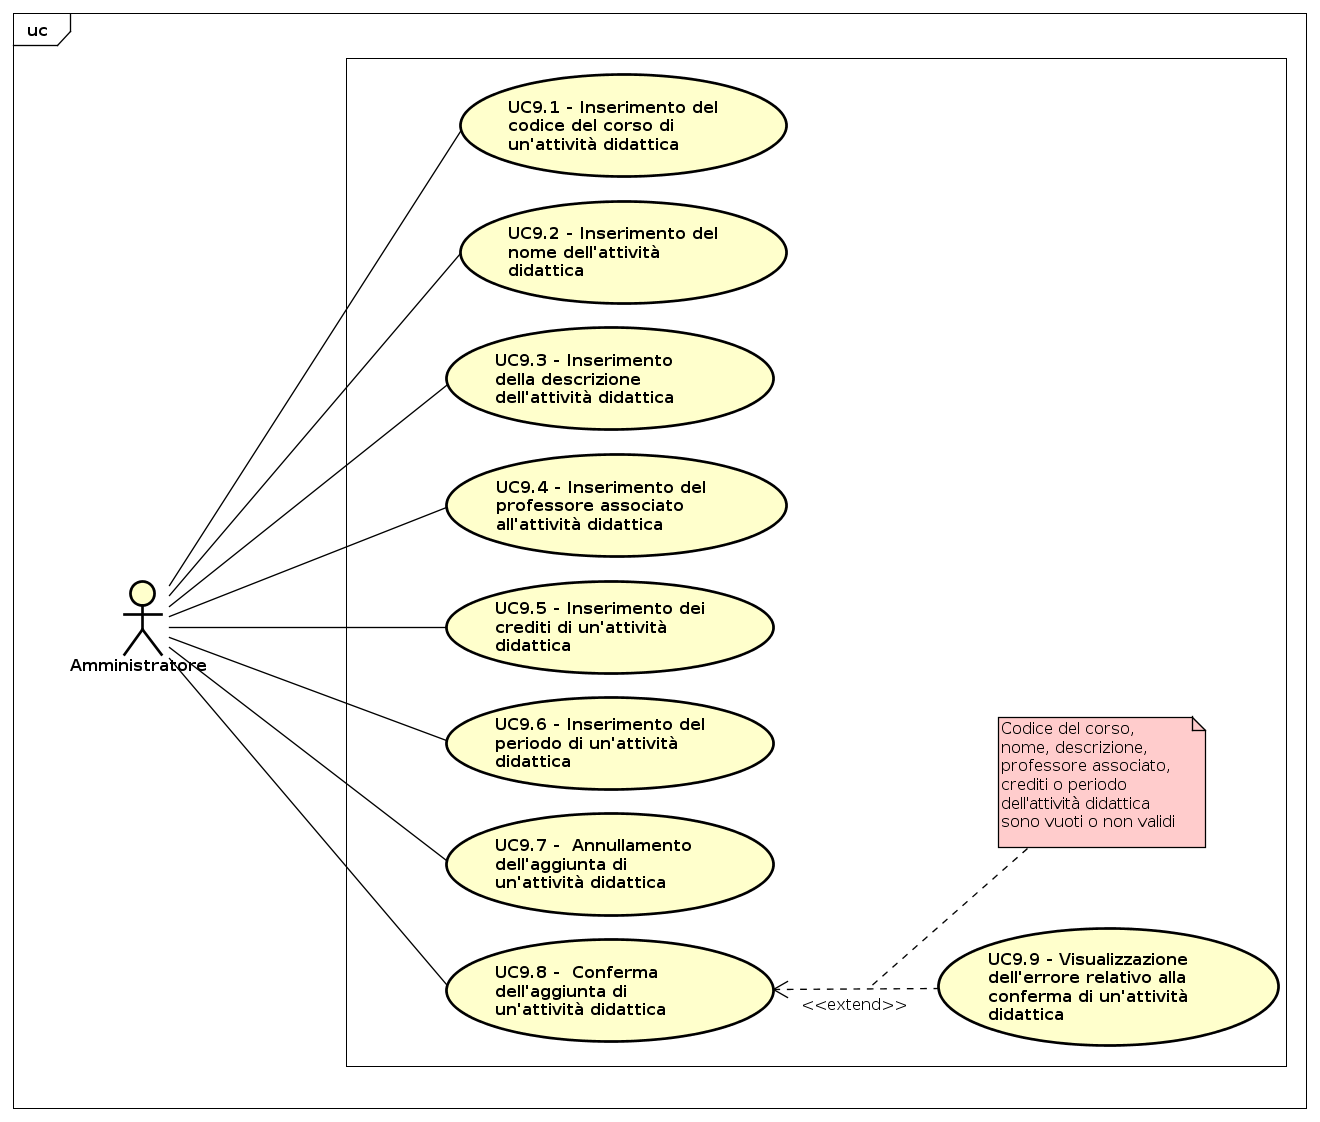
\includegraphics[scale=0.45]{./img/UseCaseDiagram09.png}
	\caption{Aggiunta di un'attività didattica}\label{}
\end{figure}
\begin{itemize}
	\item \textbf{Attori}: Amministratore, Università;
	\item \textbf{Descrizione}: L'attore aggiunge un'attività didattica alla lista delle attività didattiche;
	
	\item \textbf{Precondizione}: La lista delle attività didattiche è vuota oppure non contiene l'attività didattica che l'attore vuole inserire;
	
	\item \textbf{Flusso principale degli eventi}: L'attore, per inserire l'attività didattica alla lista, deve seguire i seguenti punti:
	\begin{itemize}
		\item Inserimento del codice del corso di un'attività didattica (UC\ref{Aggiunta di un'attivita didattica}.\ref{Inserimento del codice del corso di un'attivita didattica});
		\item Inserimento del nome di un'attività didattica (UC\ref{Aggiunta di un'attivita didattica}.\ref{Inserimento del nome di un'attivita didattica});
		\item Inserimento della descrizione di un'attività didattica (UC\ref{Aggiunta di un'attivita didattica}.\ref{Inserimento della descrizione di un'attivita didattica});
		\item Inserimento del professore associato ad un'attività didattica (UC\ref{Aggiunta di un'attivita didattica}.\ref{Inserimento del professore associato ad un'attivita didattica});
		\item Inserimento dei crediti di un'attività didattica (UC\ref{Aggiunta di un'attivita didattica}.\ref{Inserimento dei crediti di un'attivita didattica});
		\item Inserimento del periodo di un'attività didattica (UC\ref{Aggiunta di un'attivita didattica}.\ref{Inserimento del periodo di un'attivita didattica});
		\item Annullamento dell'aggiunta di un'attività didattica (UC\ref{Aggiunta di un'attivita didattica}.\ref{Annullamento dell'aggiunta di un'attivita didattica});
		\item Conferma dell'aggiunta di un'attività didattica (UC\ref{Aggiunta di un'attivita didattica}.\ref{Conferma dell'aggiunta di un'attivita didattica};
		%\item Aggiunta di un esame (UC3.6.7.9);
		\item Visualizzazione dell'errore relativo all'aggiunta di un'attività didattica non valida (UC\ref{Aggiunta di un'attivita didattica}.\ref{Visualizzazione dell'errore relativo all'aggiunta di un'attivita didattica non valida}).
	\end{itemize}
	\item \textbf{Postcondizione}: Il sistema può aver compilato dei campi relativi all'aggiunta di una nuova attività didattica.
	
\end{itemize}

%{UC3.6.7.1}
\taskOO{Inserimento del codice del corso di un'attivita didattica}
\subsection{Caso d'uso UC\ref{Aggiunta di un'attivita didattica}.\ref{Inserimento del codice del corso di un'attivita didattica}: Inserimento del codice del corso di un'attività didattica}
\begin{itemize}
	\item \textbf{Attori}: Amministratore, Università;
	\item \textbf{Descrizione}: L'attore compila il campo relativo al codice del corso dell'attività didattica;
	
	\item \textbf{Precondizione}: Il sistema fa visualizzare il campo di inserimento del codice di un'attività didattica;
	
	\item \textbf{Flusso principale degli eventi}: L'attore imposta il codice del corso dell'attività didattica;
	
	\item \textbf{Postcondizione}: È stato inserito il codice dell'attività didattica nel campo opportuno.
	
\end{itemize}

%{UC3.6.7.2}
\taskOO{Inserimento del nome di un'attivita didattica}
\subsection{Caso d'uso UC\ref{Aggiunta di un'attivita didattica}.\ref{Inserimento del nome di un'attivita didattica}: Inserimento del nome di un'attività didattica}
\begin{itemize}
	\item \textbf{Attori}: Amministratore, Università;
	\item \textbf{Descrizione}: L'attore compila il campo relativo al nome del corso dell'attività didattica;
	
	\item \textbf{Precondizione}: Il sistema fa visualizzare il campo di inserimento del nome di un'attività didattica;
	
	\item \textbf{Flusso principale degli eventi}: L'attore imposta il nome del corso dell'attività didattica;
	
	\item \textbf{Postcondizione}: È stato inserito il nome dell'attività didattica nel campo opportuno.
\end{itemize}

%{UC3.6.7.3}
\taskOO{Inserimento della descrizione di un'attivita didattica}
\subsection{Caso d'uso UC\ref{Aggiunta di un'attivita didattica}.\ref{Inserimento della descrizione di un'attivita didattica}: Inserimento della descrizione di un'attività didattica}
\begin{itemize}
	\item \textbf{Attori}: Amministratore, Università;
	\item \textbf{Descrizione}: L'attore compila il campo relativo alla descrizione dell'attività didattica;
	
	\item \textbf{Precondizione}: Il sistema fa visualizzare il campo di inserimento della descrizione di un'attività didattica;
	
	\item \textbf{Flusso principale degli eventi}: L'attore imposta la descrizione dell'attività didattica;
	
	\item \textbf{Postcondizione}: È stata inserita la descrizione dell'attività didattica nel campo opportuno.
	
\end{itemize}


%{UC3.6.7.4}
\taskOO{Inserimento del professore associato ad un'attivita didattica}
\subsection{Caso d'uso UC\ref{Aggiunta di un'attivita didattica}.\ref{Inserimento del professore associato ad un'attivita didattica}: Inserimento del professore associato ad un'attività didattica}
\begin{itemize}
	\item \textbf{Attori}: Amministratore, Università;
	\item \textbf{Descrizione}: L'attore compila il campo relativo al professore associato all'attività didattica;
	
	\item \textbf{Precondizione}: Il sistema fa visualizzare il campo di inserimento del professore associato ad un'attività didattica;
	\item \textbf{Flusso principale degli eventi}: L'attore imposta il professore associato all'attività didattica;
	
	\item \textbf{Postcondizione}: È stato inserito il professore associato all'attività didattica nel campo opportuno.
	
\end{itemize}

%{UC3.6.7.5}
\taskOO{Inserimento dei crediti di un'attivita didattica}
\subsection{Caso d'uso UC\ref{Aggiunta di un'attivita didattica}.\ref{Inserimento dei crediti di un'attivita didattica}: Inserimento dei crediti di un'attività didattica}
\begin{itemize}
	\item \textbf{Attori}: Amministratore, Università;
	\item \textbf{Descrizione}: L'attore compila il campo relativo ai crediti dell'attività didattica;
	
	\item \textbf{Precondizione}: Il sistema fa visualizzare il campo di inserimento dei crediti di un'attività didattica;
	
	\item \textbf{Flusso principale degli eventi}: L'attore imposta i crediti dell'attività didattica;
	
	\item \textbf{Postcondizione}: Sono stati inseriti i crediti dell'attività didattica nel campo opportuno.
	
\end{itemize}

%{UC3.6.7.6}
\taskOO{Inserimento del periodo di un'attivita didattica}
\subsection{Caso d'uso UC\ref{Aggiunta di un'attivita didattica}.\ref{Inserimento del periodo di un'attivita didattica}: Inserimento del periodo di un'attività didattica}
\begin{itemize}
	\item \textbf{Attori}: Amministratore, Università;
	\item \textbf{Descrizione}: L'attore compila il campo relativo al periodo dell'attività didattica;
	
	\item \textbf{Precondizione}: Il sistema fa visualizzare il campo di inserimento del periodo di un'attività didattica;
	
	\item \textbf{Flusso principale degli eventi}: L'attore imposta il periodo dell'attività didattica;
	
	\item \textbf{Postcondizione}: È stato inserito il periodo dell'attività didattica nel campo opportuno.
	
\end{itemize}

%{UC3.6.7.7}
\taskOO{Annullamento dell'aggiunta di un'attivita didattica}
\subsection{Caso d'uso UC\ref{Aggiunta di un'attivita didattica}.\ref{Annullamento dell'aggiunta di un'attivita didattica}: Annullamento dell'aggiunta di un'attività didattica}
\begin{itemize}
	\item \textbf{Attori}: Amministratore, Università;
	\item \textbf{Descrizione}: L'attore non aggiunge più un'attività didattica alla lista delle attività didattiche;
	
	\item \textbf{Precondizione}: Il sistema fa visualizzare la pagina relativa all'aggiunta di un'attività didattica;
	
	\item \textbf{Flusso principale degli eventi}: L'attore non inserisce più un'attività didattica e quindi annulla l'operazione;
	
	\item \textbf{Postcondizione}: Il sistema non aggiunge più un'attività didattica in quanto l'attore ha annullato l'operazione.
\end{itemize}

%{UC3.6.7.8}
\taskOO{Conferma dell'aggiunta di un'attivita didattica}
\subsection{Caso d'uso UC\ref{Aggiunta di un'attivita didattica}.\ref{Conferma dell'aggiunta di un'attivita didattica}: Conferma dell'aggiunta di un'attività didattica}
\begin{itemize}
	\item \textbf{Attori}: Amministratore, Università;
	\item \textbf{Descrizione}: L'attore conferma l'aggiunta di un'attività didattica alla lista delle attività didattiche;
	
	\item \textbf{Precondizione}: Il sistema fa visualizzare la pagina relativa all'aggiunta di un'attività didattica;
	
	\item \textbf{Flusso principale degli eventi}: L'attore, confermando l'inserimento dei dati, aggiunge un'attività didattica alla lista delle attività didattiche;
	
	\item \textbf{Postcondizione}: Il sistema aggiunge un'attività didattica in quanto l'attore ha confermato l'operazione;
	
	\item \textbf{Estensioni}:
	\begin{itemize}
		\item Visualizzazione dell'errore relativo all'aggiunta di un'attività didattica non valida (UC\ref{Aggiunta di un'attivita didattica}.\ref{Visualizzazione dell'errore relativo all'aggiunta di un'attivita didattica non valida}).
	\end{itemize}
\end{itemize}

%{UC3.6.7.10}
\taskOO{Visualizzazione dell'errore relativo all'aggiunta di un'attivita didattica non valida}
\subsection{Caso d'uso UC\ref{Aggiunta di un'attivita didattica}.\ref{Visualizzazione dell'errore relativo all'aggiunta di un'attivita didattica non valida}: Visualizzazione dell'errore relativo all'aggiunta di un'attività didattica non valida}
\begin{itemize}
	\item \textbf{Attori}: Amministratore, Università;
	\item \textbf{Descrizione}: L'attore aggiunge i dettagli di un'attività didattica senza rispettarne la validazione;
	
	\item \textbf{Precondizione}: Il sistema ha ricevuto campi dati errati o vuoti;
	
	\item \textbf{Flusso principale degli eventi}: L'attore, impostando in maniera errata i campi dell'attività didattica, può visualizzare uno dei seguenti errori:
	\begin{itemize}
		\item Codice del corso dell'attività didattica non valido o lasciato vuoto;
		\item Nome dell'attività didattica non valido o lasciato vuoto;
		\item Descrizione dell'attività didattica non valida o lasciato vuoto;
		\item Professore associato all'attività didattica non valido o lasciato vuoto;
		\item Crediti dell'attività didattica non validi o lasciato vuoto;
		\item Periodo dell'attività didattica non valido o lasciato vuoto;
		\item Esame associato all'attività didattica non valido o lasciato vuoto.
	\end{itemize}
	\item \textbf{Postcondizione}: Il sistema fa visualizzare un messaggio d'errore riguardante il tentativo di aggiungere un'attività didattica con campi dati errati o vuoti.
	
\end{itemize}






%{UC3.6.7.9}
\taskO{Aggiunta di un esame}
\subsection{Caso d'uso UC\ref{Aggiunta di un esame}: Aggiunta di un esame}
\begin{figure} [H]
	\centering
	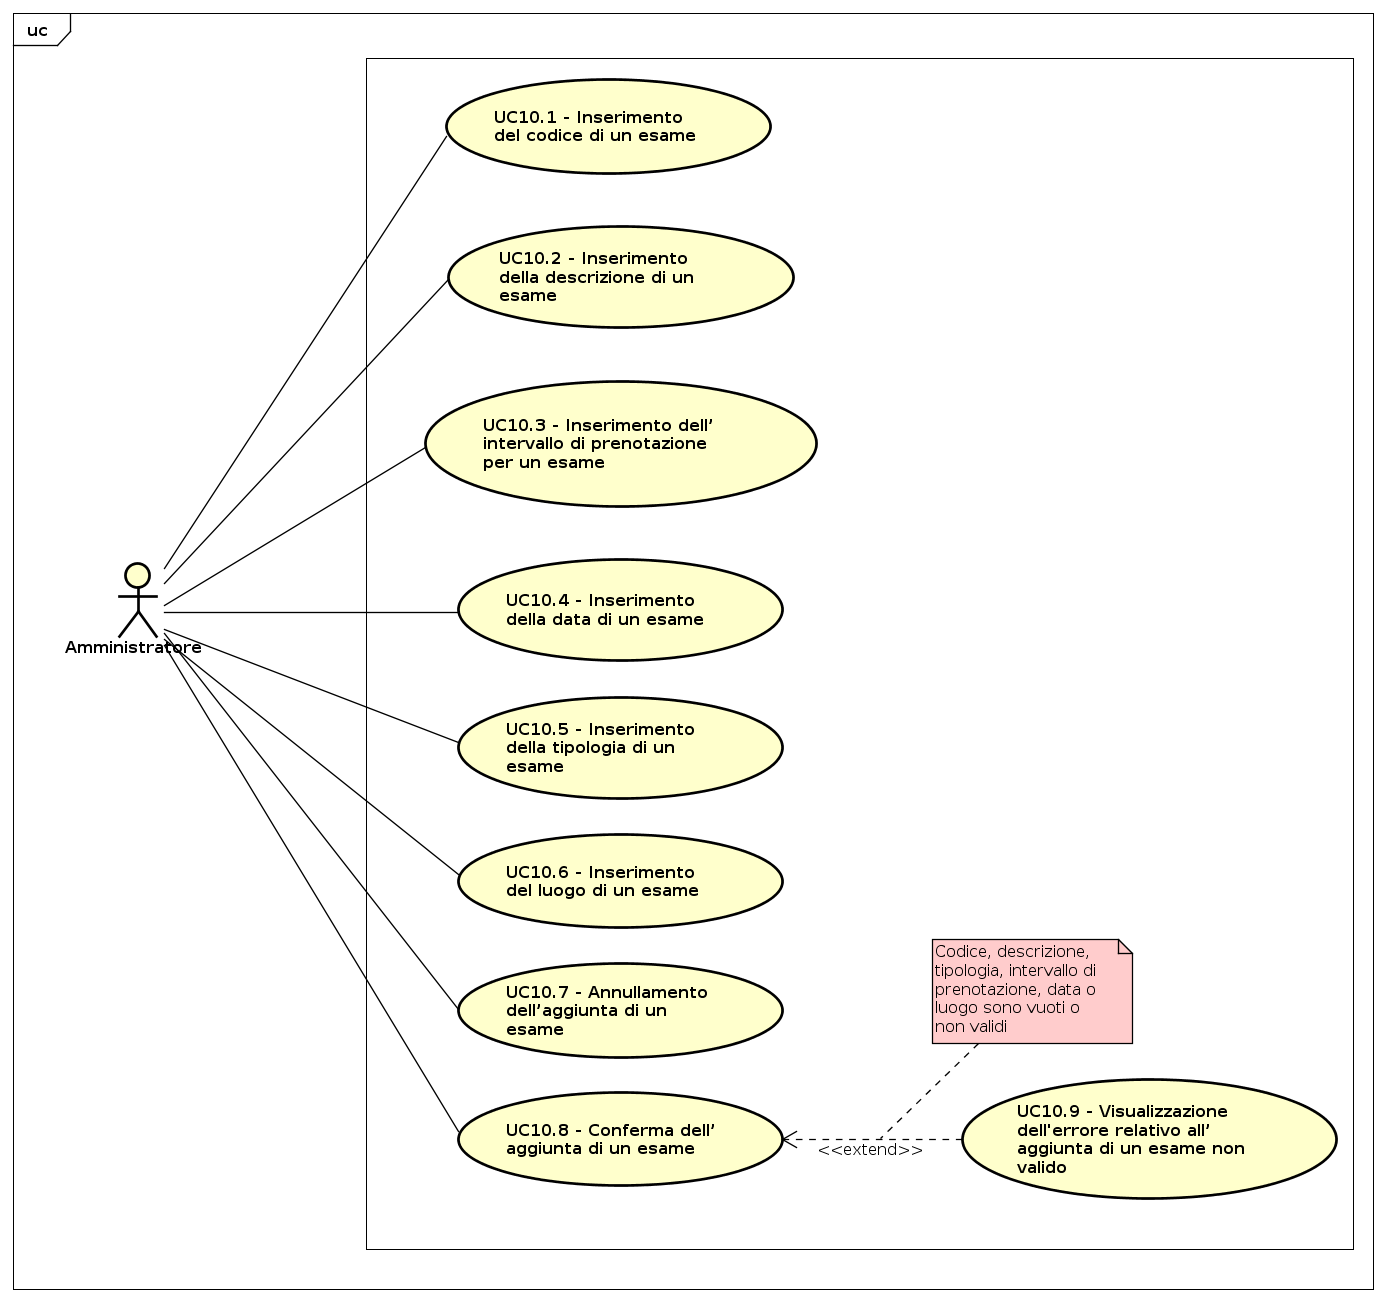
\includegraphics[scale=0.45]{./img/UseCaseDiagram010.png}
	\caption{Aggiunta di un esame}\label{}
\end{figure}
\begin{itemize}
	\item \textbf{Attori}: Amministratore, Università;
	\item \textbf{Descrizione}: L'attore aggiunge un esame alla lista degli esami;
	
	\item \textbf{Precondizione}: La lista degli esami è vuota oppure non contiene l'esame che l'attore vuole inserire;
	
	\item \textbf{Flusso principale degli eventi}: L'attore, per inserire l'esame alla lista, deve seguire i seguenti punti:
	
	\begin{itemize}
		\item Inserimento del codice di un esame (UC\ref{Aggiunta di un esame}.\ref{Inserimento del codice di un esame});
		\item Inserimento della descrizione di un esame (UC\ref{Aggiunta di un esame}.\ref{Inserimento della descrizione di un esame});
		\item Inserimento dell'intervallo di prenotazione per un esame (UC\ref{Aggiunta di un esame}.\ref{Inserimento dell'intervallo di prenotazione per un esame});
		\item Inserimento della data di un esame (UC\ref{Aggiunta di un esame}.\ref{Inserimento della data di un esame});
		\item Inserimento della tipologia di un esame (UC\ref{Aggiunta di un esame}.\ref{Inserimento della tipologia di un esame});
		\item Inserimento del luogo di un esame (UC\ref{Aggiunta di un esame}.\ref{Inserimento del luogo di un esame});
		\item Annullamento dell'aggiunta di un esame (UC\ref{Aggiunta di un esame}.\ref{Annullamento dell'aggiunta di un esame});
		\item Conferma dell'aggiunta di un esame (UC\ref{Aggiunta di un esame}.\ref{Conferma dell'aggiunta di un esame});
		\item Visualizzazione dell'errore relativo all'aggiunta di un esame non valido (UC\ref{Aggiunta di un esame}.\ref{Visualizzazione dell'errore relativo all'aggiunta di un esame non valido}).
	\end{itemize}
	\item \textbf{Postcondizione}: Il sistema può aver compilato dei campi relativi all'aggiunta di un nuovo esame;
	
\end{itemize}

%{UC3.6.7.9.1}
\taskOO{Inserimento del codice di un esame}
\subsection{Caso d'uso UC\ref{Aggiunta di un esame}.\ref{Inserimento del codice di un esame}: Inserimento del codice di un esame}
\begin{itemize}
	\item \textbf{Attori}: Amministratore, Università;
	\item \textbf{Descrizione}: L'attore compila il campo relativo al codice dell'esame;
	
	\item \textbf{Precondizione}: Il sistema fa visualizzare il campo di inserimento del codice di un esame;
	\item \textbf{Flusso principale degli eventi}: L'attore imposta il codice dell'esame;
	
	\item \textbf{Postcondizione}: È stato inserito il codice dell'esame nel campo opportuno.
\end{itemize}

%{UC3.6.7.9.2}
\taskOO{Inserimento della descrizione di un esame}
\subsection{Caso d'uso UC\ref{Aggiunta di un esame}.\ref{Inserimento della descrizione di un esame}: Inserimento della descrizione di un esame}
\begin{itemize}
	\item \textbf{Attori}: Amministratore, Università;
	\item \textbf{Descrizione}: L'attore compila il campo relativo alla descrizione dell'esame;
	
	\item \textbf{Precondizione}: Il sistema fa visualizzare il campo di inserimento della descrizione di un esame;
	\item \textbf{Flusso principale degli eventi}: L'attore aggiunge la descrizione dell'esame;
	
	\item \textbf{Postcondizione}: È stata inserita la descrizione dell'esame nel campo opportuno.
	
\end{itemize}

%{UC3.6.7.9.3}
\taskOO{Inserimento dell'intervallo di prenotazione per un esame}
\subsection{Caso d'uso UC\ref{Aggiunta di un esame}.\ref{Inserimento dell'intervallo di prenotazione per un esame}: Inserimento dell'intervallo di prenotazione per un esame}
\begin{itemize}
	\item \textbf{Attori}: Amministratore, Università;
	\item \textbf{Descrizione}: L'attore compila il campo relativo all'intervallo di prenotazione per l'esame;
	
	\item \textbf{Precondizione}: Il sistema fa visualizzare il campo di inserimento dell'intervallo di prenotazione di un esame;
	
	\item \textbf{Flusso principale degli eventi}: L'attore imposta l'intervallo di prenotazione per l'esame;
	
	\item \textbf{Postcondizione}: È stato inserito l'intervallo di prenotazione dell'esame nel campo opportuno.
	
\end{itemize}

%{UC3.6.7.9.4}
\taskOO{Inserimento della data di un esame}
\subsection{Caso d'uso UC\ref{Aggiunta di un esame}.\ref{Inserimento della data di un esame}: Inserimento della data di un esame}
\begin{itemize}
	\item \textbf{Attori}: Amministratore, Università;
	\item \textbf{Descrizione}: L'attore compila il campo relativo alla data dell'esame;
	
	\item \textbf{Precondizione}: Il sistema fa visualizzare il campo di inserimento della data di un esame;
	
	\item \textbf{Flusso principale degli eventi}: L'attore imposta la data dell'esame;
	
	\item \textbf{Postcondizione}: È stata inserita la data dell'esame nel campo opportuno.
	
\end{itemize}

%{UC3.6.7.9.5}
\taskOO{Inserimento della tipologia di un esame}
\subsection{Caso d'uso UC\ref{Aggiunta di un esame}.\ref{Inserimento della tipologia di un esame}: Inserimento della tipologia di un esame}
\begin{itemize}
	\item \textbf{Attori}: Amministratore, Università;
	\item \textbf{Descrizione}: L'attore compila il campo relativo alla tipologia dell'esame;
	
	\item \textbf{Precondizione}: Il sistema fa visualizzare il campo di inserimento della tipologia di un esame;
	
	\item \textbf{Flusso principale degli eventi}: L'attore imposta la tipologia dell'esame;
	
	\item \textbf{Postcondizione}: È stata inserita la tipologia dell'esame nel campo opportuno.
	
\end{itemize}

%{UC3.6.7.9.6}
\taskOO{Inserimento del luogo di un esame}
\subsection{Caso d'uso UC\ref{Aggiunta di un esame}.\ref{Inserimento del luogo di un esame}: Inserimento del luogo di un esame}
\begin{itemize}
	\item \textbf{Attori}: Amministratore, Università;
	\item \textbf{Descrizione}: L'attore compila il campo relativo al luogo dell'esame;
	
	\item \textbf{Precondizione}: Il sistema fa visualizzare il campo di inserimento del luogo di un esame;
	
	\item \textbf{Flusso principale degli eventi}: L'attore imposta il luogo dell'esame;
	
	\item \textbf{Postcondizione}: È stato inserito il luogo dell'esame nel campo opportuno.
	
\end{itemize}

%{UC3.6.7.9.7}
\taskOO{Annullamento dell'aggiunta di un esame}
\subsection{Caso d'uso UC\ref{Aggiunta di un esame}.\ref{Annullamento dell'aggiunta di un esame}: Annullamento dell'aggiunta di un esame}
\begin{itemize}
	\item \textbf{Attori}: Amministratore, Università;
	\item \textbf{Descrizione}: L'attore non aggiunge più un esame alla lista degli esami;
	
	\item \textbf{Precondizione}: Il sistema fa visualizzare la pagina relativa all'aggiunta di un esame;
	
	\item \textbf{Flusso principale degli eventi}: L'attore non inserisce più un esame e quindi annulla l'operazione;
	
	\item \textbf{Postcondizione}: Il sistema non aggiunge più un esame in quanto l'attore ha annullato l'operazione.
\end{itemize}

%{UC3.6.7.9.8}
\taskOO{Conferma dell'aggiunta di un esame}
\subsection{Caso d'uso UC\ref{Aggiunta di un esame}.\ref{Conferma dell'aggiunta di un esame}: Conferma dell'aggiunta di un esame}
\begin{itemize}
	\item \textbf{Attori}: Amministratore, Università;
	\item \textbf{Descrizione}: L'attore conferma l'aggiunta di un esame alla lista degli esami;
	
	\item \textbf{Precondizione}: Il sistema fa visualizzare la pagina relativa all'aggiunta di un esame;
	
	\item \textbf{Flusso principale degli eventi}: L'attore, confermando l'inserimento dei dati, aggiunge un esame alla lista degli esami;
	
	\item \textbf{Postcondizione}: Il sistema aggiunge un esame in quanto l'attore ha confermato l'operazione;
	
	\item \textbf{Estensioni}:
	\begin{itemize}
		\item Visualizzazione dell'errore relativo all'aggiunta di un esame non valido (UC\ref{Aggiunta di un esame}.\ref{Visualizzazione dell'errore relativo all'aggiunta di un esame non valido}).
	\end{itemize}
\end{itemize}

%{UC3.6.7.9.9}
\taskOO{Visualizzazione dell'errore relativo all'aggiunta di un esame non valido}
\subsection{Caso d'uso UC\ref{Aggiunta di un esame}.\ref{Visualizzazione dell'errore relativo all'aggiunta di un esame non valido}: Visualizzazione dell'errore relativo all'aggiunta di un esame non valido}
\begin{itemize}
	\item \textbf{Attori}: Amministratore, Università;
	\item \textbf{Descrizione}: L'attore aggiunge i dettagli di un esame senza rispettarne la validazione;
	
	\item \textbf{Precondizione}: Il sistema ha ricevuto campi dati errati o vuoti;
	\item \textbf{Flusso principale degli eventi}: L'attore, impostando in maniera errata i campi dell'esame, può visualizzare uno dei seguenti errori:
	\begin{itemize}
		\item Codice dell'esame non valido o lasciato vuoto;
		\item Descrizione dell'esame non valida o lasciato vuoto;
		\item Intervallo di prenotazione per l'esame non valido o lasciato vuoto;
		\item Data dell'esame non valida o lasciato vuoto;
		\item Tipologia dell'esame non valida o lasciato vuoto;
		\item Luogo d'esame non valido o lasciato vuoto.
	\end{itemize}
	\item \textbf{Postcondizione}: Il sistema fa visualizzare un messaggio d'errore riguardante il tentativo di aggiungere un esame con campi dati errati o vuoti.
	
\end{itemize}




%{UC4}
\taskO{Modifica di un anno accademico}
\subsection{Caso d'uso UC\ref{Modifica di un anno accademico}: Modifica di un anno accademico}
\begin{figure} [H]
	\centering
	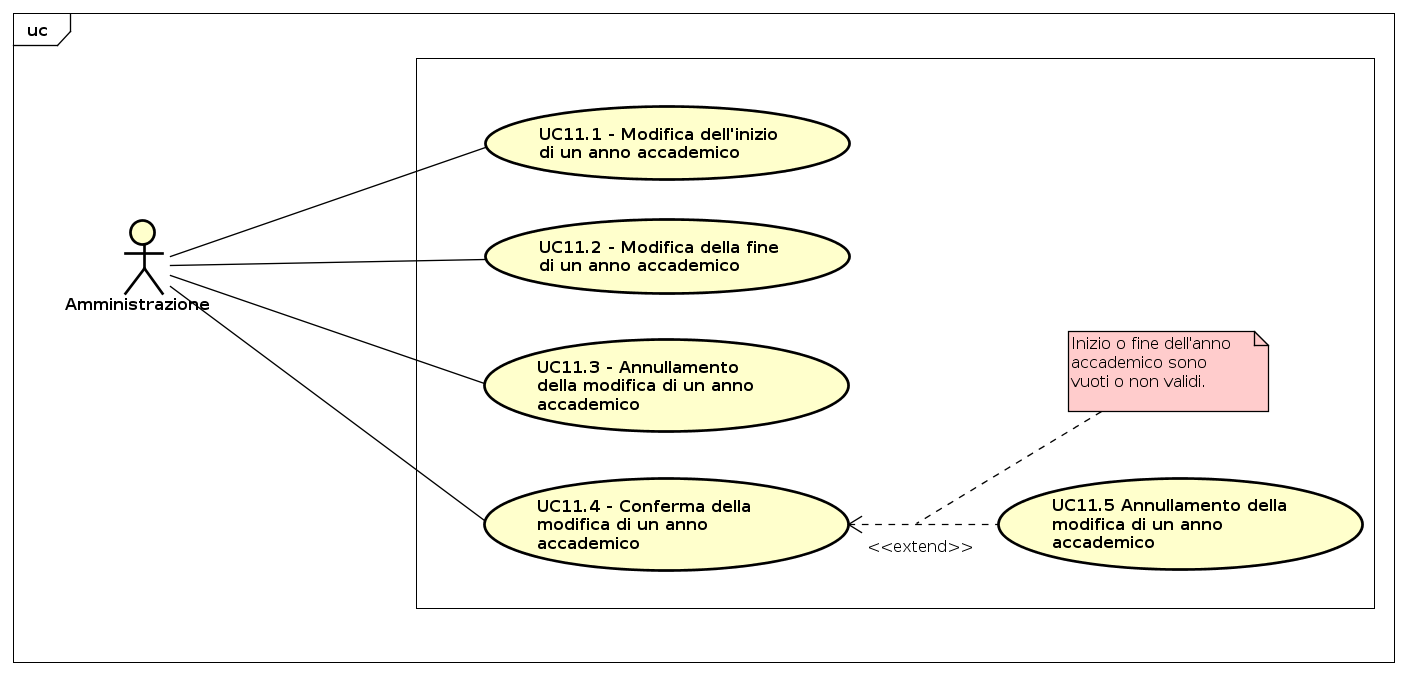
\includegraphics[scale=0.45]{./img/UseCaseDiagram011.png}
	\caption{Modifica di un anno accademico}\label{}
\end{figure}
\begin{itemize}
	\item \textbf{Attori}: Amministratore, Università;
	\item \textbf{Descrizione}: L'attore può modificare un anno accademico dalla lista degli anni accademici;
	\item \textbf{Precondizione}: Il sistema fa visualizzare un anno accademico;
	\item \textbf{Flusso principale degli eventi}: L'attore per modificare un anno accademico deve seguire i seguenti punti:
	\begin{itemize}
		\item Modifica dell'inizio di un anno accademico (UC\ref{Modifica di un anno accademico}.\ref{Modifica dell'inizio di un anno accademico});
		\item Modifica della fine di un anno accademico (UC\ref{Modifica di un anno accademico}.\ref{Modifica della fine di un anno accademico});
		\item Annullamento della modifica di un anno accademico (UC\ref{Modifica di un anno accademico}.\ref{Annullamento della modifica di un anno accademico});
		\item Conferma della modifica di un anno accademico (UC\ref{Modifica di un anno accademico}.\ref{Conferma della modifica di un anno accademico});
		\item Visualizzazione dell'errore relativo alla modifica di un anno accademico ( UC\ref{Modifica di un anno accademico}.\ref{Visualizzazione dell'errore relativo alla modifica di un anno accademico});
		%\item Modifica di un corso di laurea (UC4.6);
		%\item Eliminazione di un corso di laurea (UC4.7);
		%\item Visualizzazione dell'errore relativo all'eliminazione di un corso di laurea (UC4.8).
	\end{itemize}
	\item \textbf{Postcondizione}: Il sistema ha modificato l'anno accademico.
\end{itemize}

%{UC4.1}
\taskOO{Modifica dell'inizio di un anno accademico}
\subsection{Caso d'uso UC\ref{Modifica di un anno accademico}.\ref{Modifica dell'inizio di un anno accademico}: Modifica dell'inizio di un anno accademico}
\begin{itemize}
	\item \textbf{Attori}: Amministratore, Università;
	\item \textbf{Descrizione}: L'attore modifica la data di partenza dell'anno accademico;
	\item \textbf{Precondizione}: Il sistema fa visualizzare un anno accademico;
	\item \textbf{Flusso principale degli eventi}: L'attore modifica la data di inizio dell'anno accademico precedentemente inserita;
	\item \textbf{Postcondizione}: Il sistema ha modificato l'inizio dell'anno accademico.
\end{itemize}

%{UC4.2}
\taskOO{Modifica della fine di un anno accademico}
\subsection{Caso d'uso UC\ref{Modifica di un anno accademico}.\ref{Modifica della fine di un anno accademico}: Modifica della fine di un anno accademico}
\begin{itemize}
	\item \textbf{Attori}: Amministratore, Università;
	\item \textbf{Descrizione}: L'attore modifica la data di fine dell'anno accademico;
	\item \textbf{Precondizione}: Il sistema fa visualizzare un anno accademico;
	\item \textbf{Flusso principale degli eventi}: L'attore modifica la data di fine dell'anno accademico;
	\item \textbf{Postcondizione}: Il sistema ha modificato la data di fine dell'anno accademico.
\end{itemize}

%{UC4.3}
\taskOO{Annullamento della modifica di un anno accademico}
\subsection{Caso d'uso UC\ref{Modifica di un anno accademico}.\ref{Annullamento della modifica di un anno accademico}: Annullamento della modifica di un anno accademico}
\begin{itemize}
	\item \textbf{Attori}: Amministratore, Università;
	\item \textbf{Descrizione}: L'attore annulla la modifica dell'anno accademico;
	\item \textbf{Precondizione}: Il sistema fa visualizzare la pagina relativa alla modifica di un anno accademico;
	\item \textbf{Flusso principale degli eventi}: L'attore una volta iniziata la modifica desidera annullare il processo;
	\item \textbf{Postcondizione}: Il sistema non modifica più un anno accademico in quanto l'attore ha annullato l'operazione.
\end{itemize}

%{UC4.4}
\taskOO{Conferma della modifica di un anno accademico}
\subsection{Caso d'uso UC\ref{Modifica di un anno accademico}.\ref{Conferma della modifica di un anno accademico}: Conferma della modifica di un anno accademico}
\begin{itemize}
	\item \textbf{Attori}: Amministratore, Università;
	\item \textbf{Descrizione}: L'attore conferma la modifica relativa all'anno accademico;
	\item \textbf{Precondizione}: Il sistema fa visualizzare la pagina relativa alla modifica di un anno accademico;
	\item \textbf{Flusso principale degli eventi}: L'attore ha finito la modifica e desidera inserire nel sistema l'anno accademico modificato;
	\item \textbf{Postcondizione}: Il sistema modifica un anno accademico in quanto l'attore ha confermato l'operazione;
	\item \textbf{Estensioni}:
	\begin{itemize}
		\item Visualizzazione dell'errore relativo alla modifica di un anno accademico (UC\ref{Modifica di un anno accademico}.\ref{Visualizzazione dell'errore relativo alla modifica di un anno accademico}).
	\end{itemize}
\end{itemize}

%{UC4.5}
\taskOO{Visualizzazione dell'errore relativo alla modifica di un anno accademico}
\subsection{Caso d'uso UC\ref{Modifica di un anno accademico}.\ref{Visualizzazione dell'errore relativo alla modifica di un anno accademico}: Visualizzazione dell'errore relativo alla modifica di un anno accademico}
\begin{itemize}
	\item \textbf{Attori}: Amministratore, Università;
	\item \textbf{Descrizione}: L'attore può visualizzare un errore nel caso avesse modificato erroneamente dei campi dati;
	\item \textbf{Precondizione}: Il sistema ha ricevuto campi dati errati o vuoti;
	\item \textbf{Flusso principale degli eventi}: L'attore, modificando in maniera errata i campi dell'anno accademico, può visualizzare uno dei seguenti errori: 
	\begin{itemize}
		\item Inizio dell'anno accademico non valido o lasciato vuoto; 
		\item Fine dell'anno accademico non valido o lasciato vuoto; 
		\item Nome dell'anno accademico non valido o lasciato vuoto. 
	\end{itemize}
	\item \textbf{Postcondizione}: Il sistema visualizza un messaggio d'errore relativo all'operazione di modifica di un anno accademico.
\end{itemize}








%{UC4.6}
\taskO{Modifica di un corso di laurea}
\subsection{Caso d'uso UC\ref{Modifica di un corso di laurea}: Modifica di un corso di laurea}
\begin{figure} [H]
	\centering
	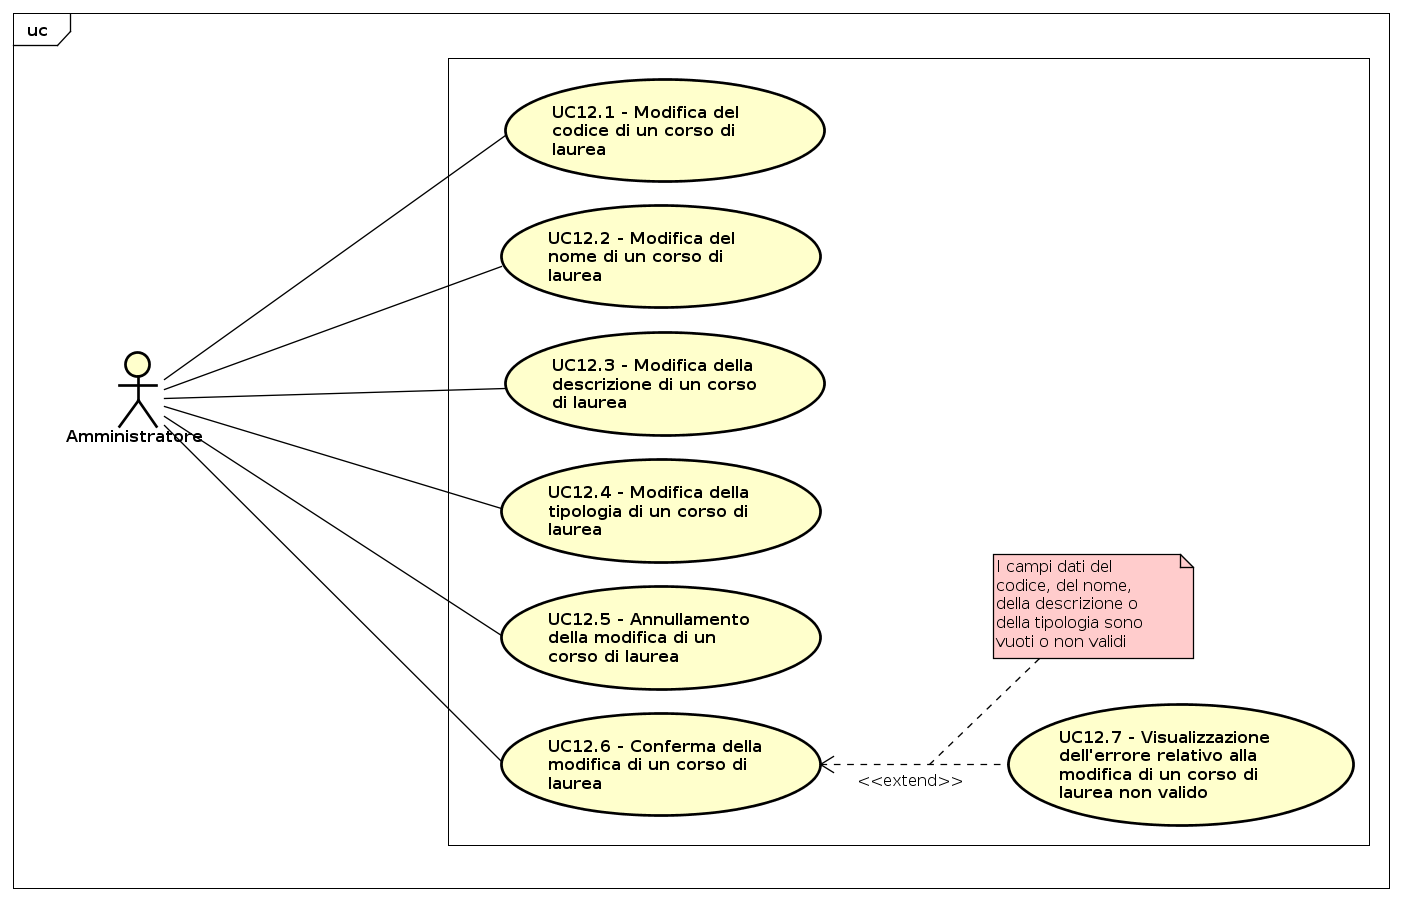
\includegraphics[scale=0.45]{./img/UseCaseDiagram012.png}
	\caption{Modifica di un corso di laurea}\label{}
\end{figure}
\begin{itemize}
	\item \textbf{Attori}: Amministratore, Università;
	\item \textbf{Descrizione}: L'attore può modificare un corso di laurea dalla lista dei corsi di laurea;
	
	\item \textbf{Precondizione}: Il sistema fa visualizzare un corso di laurea;
	
	\item \textbf{Flusso principale degli eventi}: L'attore per modificare un corso di laurea deve seguire i seguenti punti:
	
	\begin{itemize}
		\item Modifica del codice di un corso di laurea (UC\ref{Modifica di un corso di laurea}.\ref{Modifica del codice di un corso di laurea});
		\item Modifica del nome di un corso di laurea (UC\ref{Modifica di un corso di laurea}.\ref{Modifica del nome di un corso di laurea});
		\item Modifica della descrizione di un corso di laurea (UC\ref{Modifica di un corso di laurea}.\ref{Modifica della descrizione di un corso di laurea});
		\item Modifica della tipologia di un corso di laurea (UC\ref{Modifica di un corso di laurea}.\ref{Modifica della tipologia di un corso di laurea});
		\item Annullamento della modifica di un corso di laurea (UC\ref{Modifica di un corso di laurea}.\ref{Annullamento della modifica di un corso di laurea});
		\item Conferma della modifica di un corso di laurea (UC\ref{Modifica di un corso di laurea}.\ref{Conferma della modifica di un corso di laurea});
		\item Visualizzazione dell'errore relativo alla modifica di un corso di laurea non valido (UC\ref{Modifica di un corso di laurea}.\ref{Visualizzazione dell'errore relativo alla modifica di un corso di laurea non valido});
		%\item Modifica di un'attività didattica (UC4.6.8);
		%\item Eliminazione di un'attività didattica (UC4.6.9);
		%\item Visualizzazione dell'errore relativo all'eliminazione di un'attività didattica (UC4.6.10).
	\end{itemize}
	\item \textbf{Postcondizione}: Il sistema ha modificato il corso di laurea.
	
\end{itemize}

%{UC4.6.1}
\taskOO{Modifica del codice di un corso di laurea}
\subsection{Caso d'uso UC\ref{Modifica di un corso di laurea}.\ref{Modifica del codice di un corso di laurea}: Modifica del codice di un corso di laurea}
\begin{itemize}
	\item \textbf{Attori}: Amministratore, Università;
	\item \textbf{Descrizione}: L'attore modifica il codice del corso di laurea;
	
	\item \textbf{Precondizione}: Il sistema fa visualizzare il campo di modifica del codice di un corso di laurea;
	\item \textbf{Flusso principale degli eventi}: L'attore modifica il codice del corso di laurea precedentemente inserito;
	
	\item \textbf{Postcondizione}: È stato modificato il codice del corso di laurea nel campo opportuno.
	
	
\end{itemize}

%{UC4.6.2}
\taskOO{Modifica del nome di un corso di laurea}
\subsection{Caso d'uso UC\ref{Modifica di un corso di laurea}.\ref{Modifica del nome di un corso di laurea}: Modifica del nome di un corso di laurea}
\begin{itemize}
	\item \textbf{Attori}: Amministratore, Università;
	\item \textbf{Descrizione}: L'attore modifica il nome del corso di laurea;
	
	\item \textbf{Precondizione}: Il sistema fa visualizzare il campo di modifica del nome di un corso di laurea;
	
	\item \textbf{Flusso principale degli eventi}: L'attore modifica il nome del corso di laurea precedentemente inserito;
	
	\item \textbf{Postcondizione}: È stato modificato il nome del corso di laurea nel campo opportuno.
	
	
\end{itemize}

%{UC4.6.3}
\taskOO{Modifica della descrizione di un corso di laurea}
\subsection{Caso d'uso UC\ref{Modifica di un corso di laurea}.\ref{Modifica della descrizione di un corso di laurea}: Modifica della descrizione di un corso di laurea}
\begin{itemize}
	\item \textbf{Attori}: Amministratore, Università;
	\item \textbf{Descrizione}: L'attore modifica la descrizione del corso di laurea;
	
	\item \textbf{Precondizione}: Il sistema fa visualizzare il campo di modifica della descrizione di un corso di laurea;
	
	\item \textbf{Flusso principale degli eventi}: L'attore modifica la descrizione del corso di laurea precedentemente inserita;
	
	\item \textbf{Postcondizione}: È stata modificata la descrizione del corso di laurea nel campo opportuno.
	
\end{itemize}

%{UC4.6.4}
\taskOO{Modifica della tipologia di un corso di laurea}
\subsection{Caso d'uso UC\ref{Modifica di un corso di laurea}.\ref{Modifica della tipologia di un corso di laurea}: Modifica della tipologia di un corso di laurea}
\begin{itemize}
	\item \textbf{Attori}: Amministratore, Università;
	\item \textbf{Descrizione}: L'attore modifica la tipologia del corso di laurea;
	
	\item \textbf{Precondizione}: Il sistema fa visualizzare il campo di modifica della tipologia di un corso di laurea;
	
	\item \textbf{Flusso principale degli eventi}: L'attore modifica la tipologia del corso di laurea precedentemente inserito;
	
	\item \textbf{Postcondizione}: È stata modificata la tipologia del corso di laurea nel campo opportuno.
	
\end{itemize}

%{UC4.6.5}
\taskOO{Annullamento della modifica di un corso di laurea}
\subsection{Caso d'uso UC\ref{Modifica di un corso di laurea}.\ref{Annullamento della modifica di un corso di laurea}: Annullamento della modifica di un corso di laurea}
\begin{itemize}
	\item \textbf{Attori}: Amministratore, Università;
	\item \textbf{Descrizione}: L'attore annulla la modifica del corso di laurea;
	
	\item \textbf{Precondizione}: l sistema fa visualizzare la pagina relativa alla modifica di un corso di laurea;
	
	\item \textbf{Flusso principale degli eventi}: L'attore una volta iniziata la modifica desidera annullare il processo;
	
	\item \textbf{Postcondizione}: Il sistema non modifica più un corso di laurea in quanto l'attore ha annullato l'operazione.
	
\end{itemize}

%{UC4.6.6}
\taskOO{Conferma della modifica di un corso di laurea}
\subsection{Caso d'uso UC\ref{Modifica di un corso di laurea}.\ref{Conferma della modifica di un corso di laurea}: Conferma della modifica di un corso di laurea}
\begin{itemize}
	\item \textbf{Attori}: Amministratore, Università;
	\item \textbf{Descrizione}: L'attore conferma la modifica relativa al corso di laurea;
	
	\item \textbf{Precondizione}: Il sistema fa visualizzare la pagina relativa alla modifica di un corso di laurea;
	
	
	\item \textbf{Flusso principale degli eventi}: L'attore ha finito la modifica e desidera inserire nel sistema il corso di laurea modificato;
	
	\item \textbf{Postcondizione}: Il sistema modifica un corso di laurea in quanto l'attore ha confermato l'operazione;
	
	\item \textbf{Estensioni}:
	\begin{itemize}
		\item Visualizzazione dell'errore relativo alla modifica di un corso di laurea non valido (UC4.6.7);
	\end{itemize}
\end{itemize}

%{UC4.6.7}
\taskOO{Visualizzazione dell'errore relativo alla modifica di un corso di laurea non valido}
\subsection{Caso d'uso UC\ref{Modifica di un corso di laurea}.\ref{Visualizzazione dell'errore relativo alla modifica di un corso di laurea non valido}: Visualizzazione dell'errore relativo alla modifica di un corso di laurea non valido}
\begin{itemize}
	\item \textbf{Attori}: Amministratore, Università;
	\item \textbf{Descrizione}: Il sistema visualizza un messaggio d'errore riguardante l'impossibilità di modificare un corso di laurea;
	
	\item \textbf{Precondizione}: Il sistema durante l'operazione di modifica ha ricevuto campi dati errati o vuoti;
	
	\item \textbf{Flusso principale degli eventi}: L'attore, modificando in maniera errata i campi del corso di laurea, può visualizzare uno dei seguenti errori: 
	\begin{itemize} 
		\item Codice del corso di laurea non valido o lasciato vuoto; 
		\item Nome del corso di laurea non valido o lasciato vuoto; 
		\item Descrizione del corso di laurea non valido o lasciato vuoto; 
		\item Codice del corso di laurea non valido o lasciato vuoto; 
		\item Tipologia del corso di laurea non valido o lasciato vuoto; 
		\item Codice dell'anno accademico non valido o lasciato vuoto; 
		\item Attività didattica del corso di laurea non valida o lasciata vuota.
	\end{itemize}
	\item \textbf{Postcondizione}: Il sistema fa visualizzare un messaggio d'errore riguardante il tentativo di modificare un corso di laurea con campi dati errati o vuoti.
	
\end{itemize}





%{UC4.6.8}
\taskO{Modifica di un'attivita didattica}
\subsection{Caso d'uso UC\ref{Modifica di un'attivita didattica}: Modifica di un'attività didattica}
\begin{figure} [H]
	\centering
	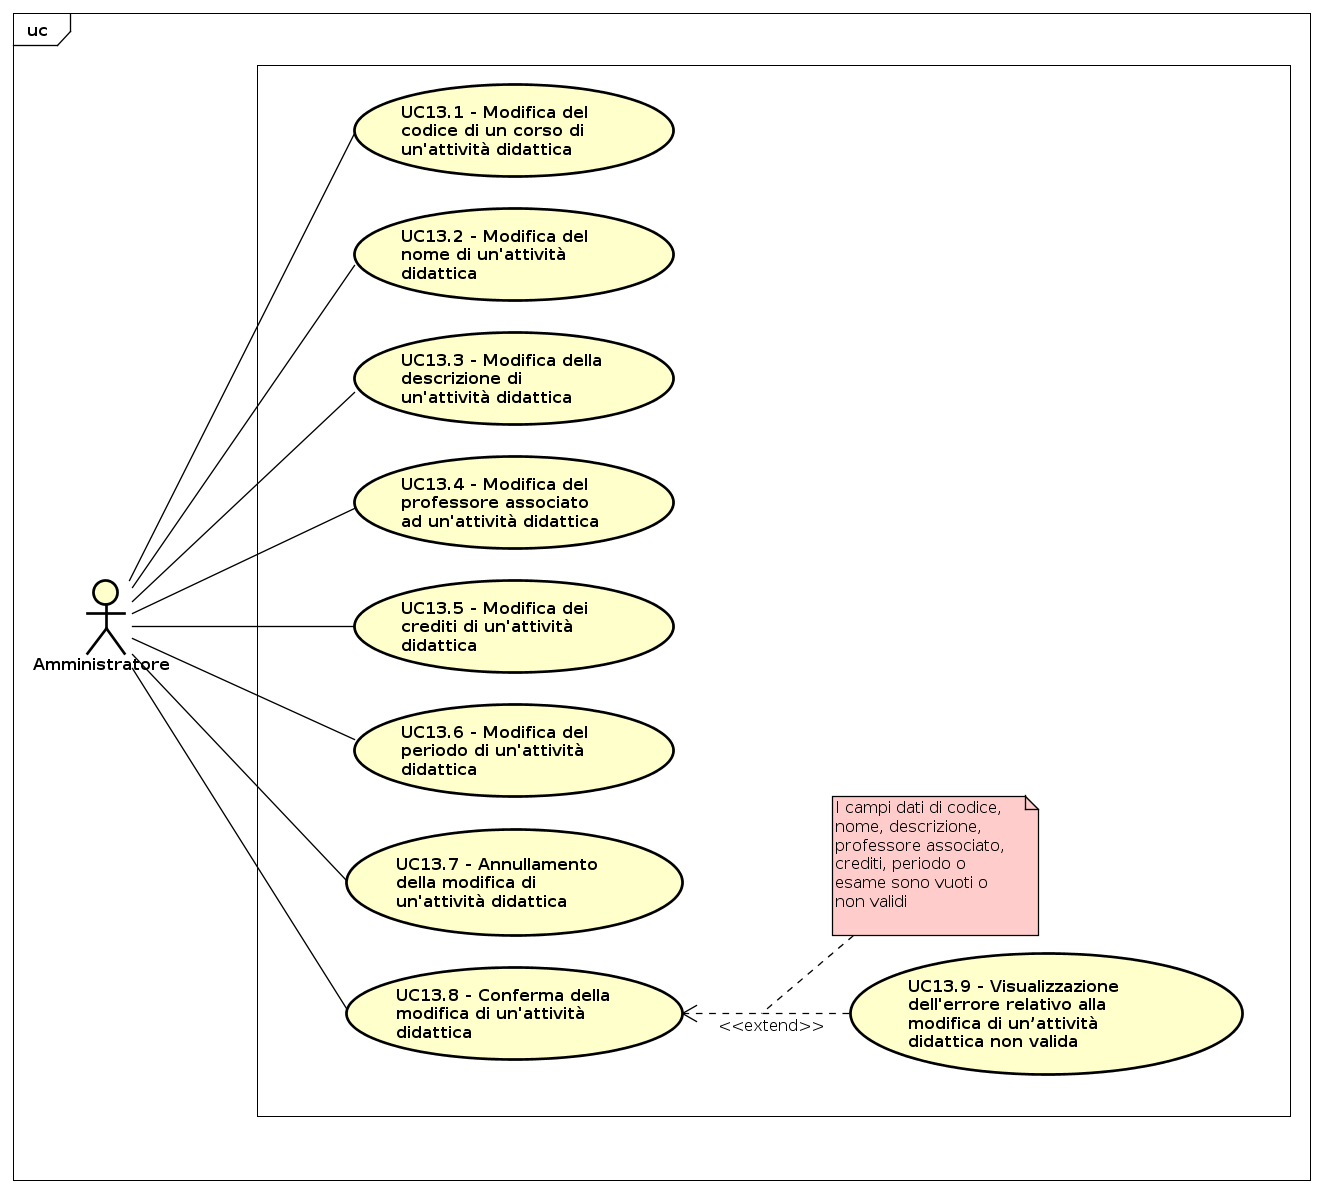
\includegraphics[scale=0.45]{./img/UseCaseDiagram013.png}
	\caption{Modifica di un'attività didattica}\label{}
\end{figure}
\begin{itemize}
	\item \textbf{Attori}: Amministratore, Università;
	\item \textbf{Descrizione}: L'attore può modificare un'attività didattica dalla lista delle attività didattiche;
	
	\item \textbf{Precondizione}: Il sistema fa visualizzare un'attività didattica;
	
	\item \textbf{Flusso principale degli eventi}: L'attore per modificare un'attività didattica deve seguire i seguenti punti:
	
	\begin{itemize}
		\item Modifica del codice di un'attività didattica (UC\ref{Modifica di un'attivita didattica}.\ref{Modifica del codice di un'attivita didattica});
		\item Modifica del nome di un'attività didattica (UC\ref{Modifica di un'attivita didattica}.\ref{Modifica del nome di un'attivita didattica});
		\item Modifica della descrizione di un'attività didattica (UC\ref{Modifica di un'attivita didattica}.\ref{Modifica della descrizione di un'attivita didattica});
		\item Modifica del professore associato ad un'attività didattica (UC\ref{Modifica di un'attivita didattica}.\ref{Modifica del professore associato ad un'attivita didattica});
		\item Modifica dei crediti di un'attività didattica (UC\ref{Modifica di un'attivita didattica}.\ref{Modifica dei crediti di un'attivita didattica});
		\item Modifica del periodo di un'attività didattica (UC\ref{Modifica di un'attivita didattica}.\ref{Modifica del periodo di un'attivita didattica});
		\item Annullamento della modifica di un'attività didattica (UC\ref{Modifica di un'attivita didattica}.\ref{Annullamento della modifica di un'attivita didattica});
		\item Conferma della modifica di un'attività didattica (UC\ref{Modifica di un'attivita didattica}.\ref{Conferma della modifica di un'attivita didattica});
		\item Visualizzazione dell'errore relativo alla modifica di un'attività didattica non valida (UC\ref{Modifica di un'attivita didattica}.\ref{Visualizzazione dell'errore relativo alla modifica di un'attivita didattica non valida});
		%\item Modifica di un esame (UC4.6.8.10);
		%\item Eliminazione di un esame (UC4.6.8.11);
		%\item Visualizzazione dell'errore relativo all'eliminazione di un esame (UC4.6.8.12).
	\end{itemize}
	\item \textbf{Postcondizione}: Il sistema ha modificato un'attività didattica.
	
\end{itemize}

%{UC4.6.8.1}
\taskOO{Modifica del codice di un'attivita didattica}
\subsection{Caso d'uso UC\ref{Modifica di un'attivita didattica}.\ref{Modifica del codice di un'attivita didattica}: Modifica del codice di un'attività didattica}
\begin{itemize}
	\item \textbf{Attori}: Amministratore, Università;
	\item \textbf{Descrizione}: L'attore modifica il codice di un'attività didattica;
	
	\item \textbf{Precondizione}: Il sistema fa visualizzare l'attività didattica;
	
	\item \textbf{Flusso principale degli eventi}: L'attore modifica il codice dell'attività didattica precedentemente inserito;
	
	\item \textbf{Postcondizione}: Il sistema ha modificato il codice dell'attività didattica.
	
\end{itemize}

%{UC4.6.8.2}
\taskOO{Modifica del nome di un'attivita didattica}
\subsection{Caso d'uso UC\ref{Modifica di un'attivita didattica}.\ref{Modifica del nome di un'attivita didattica}: Modifica del nome di un'attività didattica}
\begin{itemize}
	\item \textbf{Attori}: Amministratore, Università;
	\item \textbf{Descrizione}: L'attore modifica il nome di un'attività didattica;
	
	\item \textbf{Precondizione}: Il sistema fa visualizzare un'attività didattica;
	
	
	\item \textbf{Flusso principale degli eventi}: L'attore modifica il nome di un'attività didattica precedentemente inserito;
	
	\item \textbf{Postcondizione}: Il sistema ha modificato il nome di un'attività didattica.
	
\end{itemize}

%{UC4.6.8.3}
\taskOO{Modifica della descrizione di un'attivita didattica}
\subsection{Caso d'uso UC\ref{Modifica di un'attivita didattica}.\ref{Modifica della descrizione di un'attivita didattica}: Modifica della descrizione di un'attività didattica}
\begin{itemize}
	\item \textbf{Attori}: Amministratore, Università;
	\item \textbf{Descrizione}: L'attore modifica la descrizione di un'attività didattica;
	
	\item \textbf{Precondizione}: Il sistema fa visualizzare un'attività didattica;
	
	
	\item \textbf{Flusso principale degli eventi}: L'attore modifica la descrizione di un'attività didattica precedentemente inserita;
	
	\item \textbf{Postcondizione}: Il sistema ha modificato la descrizione di un'attività didattica.
	
\end{itemize}

%{UC4.6.8.4}
\taskOO{Modifica del professore associato ad un'attivita didattica}
\subsection{Caso d'uso UC\ref{Modifica di un'attivita didattica}.\ref{Modifica del professore associato ad un'attivita didattica}: Modifica del professore associato ad un'attività didattica}
\begin{itemize}
	\item \textbf{Attori}: Amministratore, Università;
	\item \textbf{Descrizione}: L'attore modifica il professore associato ad un'attività didattica;
	
	\item \textbf{Precondizione}: Il sistema fa visualizzare un'attività didattica;
	
	
	\item \textbf{Flusso principale degli eventi}: L'attore modifica il professore associato ad un'attività didattica precedentemente inserito;
	
	\item \textbf{Postcondizione}: Il sistema ha modificato il professore associato ad un'attività didattica.
	
\end{itemize}

%{UC4.6.8.5}
\taskOO{Modifica dei crediti di un'attivita didattica}
\subsection{Caso d'uso UC\ref{Modifica di un'attivita didattica}.\ref{Modifica dei crediti di un'attivita didattica}: Modifica dei crediti di un'attività didattica}
\begin{itemize}
	\item \textbf{Attori}: Amministratore, Università;
	\item \textbf{Descrizione}: L'attore modifica i crediti di un'attività didattica;
	
	\item \textbf{Precondizione}: Il sistema fa visualizzare un'attività didattica;
	
	
	\item \textbf{Flusso principale degli eventi}: L'attore modifica i crediti di un'attività didattica precedentemente inseriti;
	
	\item \textbf{Postcondizione}: Il sistema ha modificato i crediti di un'attività didattica.
	
\end{itemize}

%{UC4.6.8.6}
\taskOO{Modifica del periodo di un'attivita didattica}
\subsection{Caso d'uso UC\ref{Modifica di un'attivita didattica}.\ref{Modifica del periodo di un'attivita didattica}: Modifica del periodo di un'attività didattica}
\begin{itemize}
	\item \textbf{Attori}: Amministratore, Università;
	\item \textbf{Descrizione}: L'attore modifica il periodo di un'attività didattica;
	
	\item \textbf{Precondizione}: Il sistema fa visualizzare un'attività didattica;
	
	
	\item \textbf{Flusso principale degli eventi}: L'attore modifica il periodo di un'attività didattica precedentemente inserito;
	
	\item \textbf{Postcondizione}: Il sistema ha modificato il periodo di un'attività didattica.
	
\end{itemize}

%{UC4.6.8.7}
\taskOO{Annullamento della modifica di un'attivita didattica}
\subsection{Caso d'uso UC\ref{Modifica di un'attivita didattica}.\ref{Annullamento della modifica di un'attivita didattica}: Annullamento della modifica di un'attività didattica}
\begin{itemize}
	\item \textbf{Attori}: Amministratore, Università;
	\item \textbf{Descrizione}: L'attore annulla la di un'attività didattica;
	
	\item \textbf{Precondizione}: Il sistema fa visualizzare la pagina relativa alla modifica di un'attività didattica;
	
	\item \textbf{Flusso principale degli eventi}: L'attore una volta iniziata la modifica desidera annullare il processo;
	
	\item \textbf{Postcondizione}: Il sistema non modifica più un'attività didattica in quanto l'attore ha annullato l'operazione.
	
\end{itemize}

%{UC4.6.8.8}
\taskOO{Conferma della modifica di un'attivita didattica}
\subsection{Caso d'uso UC\ref{Modifica di un'attivita didattica}.\ref{Conferma della modifica di un'attivita didattica}: Conferma della modifica di un'attività didattica}
\begin{itemize}
	\item \textbf{Attori}: Amministratore, Università;
	\item \textbf{Descrizione}: L'attore conferma la modifica relativa ad un'attività didattica;
	
	\item \textbf{Precondizione}: Il sistema fa visualizzare la pagina relativa alla modifica di un'attività didattica;
	
	
	\item \textbf{Flusso principale degli eventi}: L'attore ha finito la modifica e desidera inserire nel sistema l'attività didattica modificata;
	
	\item \textbf{Postcondizione}: Il sistema modifica un'attività didattica in quanto l'attore ha confermato l'operazione;
	
	
	\item \textbf{Estensioni}:
	\begin{itemize}
		\item Visualizzazione dell'errore relativo alla modifica di un'attività didattica non valida (UC\ref{Modifica di un'attivita didattica}.\ref{Visualizzazione dell'errore relativo alla modifica di un'attivita didattica non valida}).
	\end{itemize}
\end{itemize}

%{UC4.6.8.9}
\taskOO{Visualizzazione dell'errore relativo alla modifica di un'attivita didattica non valida}
\subsection{Caso d'uso UC\ref{Modifica di un'attivita didattica}.\ref{Visualizzazione dell'errore relativo alla modifica di un'attivita didattica non valida}: Visualizzazione dell'errore relativo alla modifica di un'attività didattica non valida}
\begin{itemize}
	\item \textbf{Attori}: Amministratore, Università;
	\item \textbf{Descrizione}: Il sistema visualizza un messaggio d'errore riguardante l'impossibilità di modificare di un'attività didattica;
	
	\item \textbf{Precondizione}: Il sistema ha ricevuto campi dati errati o vuoti;
	
	\item \textbf{Flusso principale degli eventi}: L'attore, modificando in maniera errata i campi di un'attività didattica, può visualizzare uno dei seguenti errori: 
	\begin{itemize} 
		\item Codice del corso dell'attività didattica non valido o lasciato vuoto; 
		\item Nome dell'attività didattica non valido o lasciato vuoto;
		\item Descrizione dell'attività didattica non valida o lasciato vuoto; 
		\item Professore associato all'attività didattica non valido o lasciato vuoto;
		\item Crediti dell'attività didattica non validi o lasciato vuoto; 
		\item Periodo dell'attività didattica non valido o lasciato vuoto; 
		\item Esame associato all'attività didattica non valido o lasciato vuoto. 
	\end{itemize}
	\item \textbf{Postcondizione}: Il sistema visualizza un messaggio d'errore relativo all'operazione di modifica di un'attività didattica.
	
	
\end{itemize}





%{UC4.6.8.10}
\taskO{Modifica di un esame}
\subsection{Caso d'uso UC\ref{Modifica di un esame}: Modifica di un esame}
\begin{figure} [H]
	\centering
	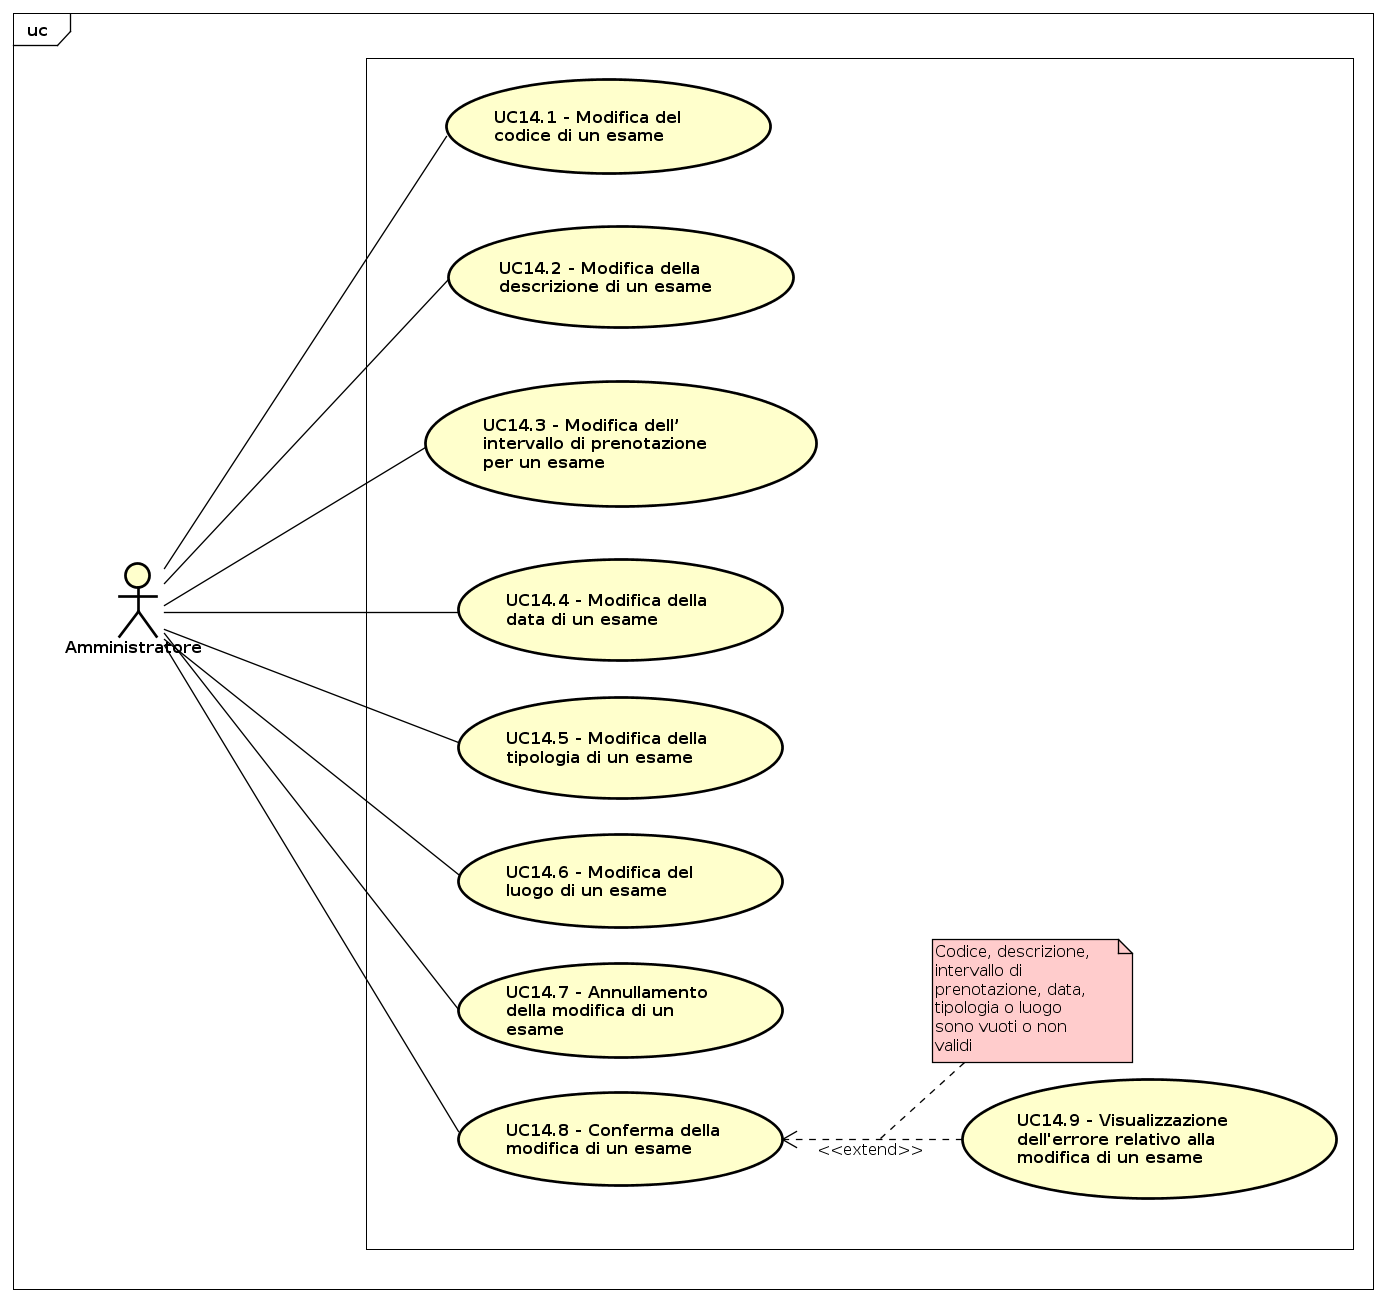
\includegraphics[scale=0.45]{./img/UseCaseDiagram014.png}
	\caption{Modifica di un esame}\label{}
\end{figure}
\begin{itemize}
	\item \textbf{Attori}: Amministratore, Università;
	\item \textbf{Descrizione}: L'attore può modificare un esame dalla lista degli esami;
	
	\item \textbf{Precondizione}: Il sistema fa visualizzare un esame;
	
	\item \textbf{Flusso principale degli eventi}: L'attore per modificare un esame deve seguire i seguenti punti:
	
	\begin{itemize}
		\item Modifica del codice di un esame (UC\ref{Modifica di un esame}.\ref{Modifica del codice di un esame});
		\item Modifica della descrizione di un esame (UC\ref{Modifica di un esame}.\ref{Modifica della descrizione di un esame});
		\item Modifica dell'intervallo di prenotazione di un esame (UC\ref{Modifica di un esame}.\ref{Modifica dell'intervallo di prenotazione di un esame});
		\item Modifica della data di un esame (UC\ref{Modifica di un esame}.\ref{Modifica della data di un esame});
		\item Modifica della tipologia di un esame (UC\ref{Modifica di un esame}.\ref{Modifica della tipologia di un esame});
		\item Modifica del luogo di un esame (UC\ref{Modifica di un esame}.\ref{Modifica del luogo di un esame});
		\item Annullamento della modifica di un esame (UC\ref{Modifica di un esame}.\ref{Annullamento della modifica di un esame});
		\item Conferma della modifica di un esame (UC\ref{Modifica di un esame}.\ref{Conferma della modifica di un esame});
		\item Visualizzazione dell'errore relativo alla modifica di un esame (UC\ref{Modifica di un esame}.\ref{Visualizzazione dell'errore relativo alla modifica di un esame}).
	\end{itemize}
	\item \textbf{Postcondizione}: Il sistema ha modificato l'esame.
	
\end{itemize}

%{UC4.6.8.10.1}
\taskOO{Modifica del codice di un esame}
\subsection{Caso d'uso UC\ref{Modifica di un esame}.\ref{Modifica del codice di un esame}: Modifica del codice di un esame}
\begin{itemize}
	\item \textbf{Attori}: Amministratore, Università;
	\item \textbf{Descrizione}: L'attore modifica il codice di un esame;
	
	\item \textbf{Precondizione}: Il sistema fa visualizzare un esame;
	
	
	\item \textbf{Flusso principale degli eventi}: L'attore modifica il codice di un esame precedentemente inserito;
	
	\item \textbf{Postcondizione}: Il sistema ha modificato il codice dell'esame.
	
\end{itemize}

%{UC4.6.8.10.2}
\taskOO{Modifica della descrizione di un esame}
\subsection{Caso d'uso UC\ref{Modifica di un esame}.\ref{Modifica della descrizione di un esame}: Modifica della descrizione di un esame}
\begin{itemize}
	\item \textbf{Attori}: Amministratore, Università;
	\item \textbf{Descrizione}: L'attore modifica la descrizione di un esame;
	
	\item \textbf{Precondizione}: Il sistema fa visualizzare un esame;
	
	\item \textbf{Flusso principale degli eventi}: L'attore modifica la descrizione dell'esame precedentemente inserita;
	
	\item \textbf{Postcondizione}: Il sistema ha modificato la descrizione dell'esame.
	
\end{itemize}

%{UC4.6.8.10.3}
\taskOO{Modifica dell'intervallo di prenotazione di un esame}
\subsection{Caso d'uso UC\ref{Modifica di un esame}.\ref{Modifica dell'intervallo di prenotazione di un esame}: Modifica dell'intervallo di prenotazione di un esame}
\begin{itemize}
	\item \textbf{Attori}: Amministratore, Università;
	\item \textbf{Descrizione}: L'attore modifica l'intervallo di prenotazione di un esame;
	
	\item \textbf{Precondizione}: Il sistema fa visualizzare un esame;
	
	\item \textbf{Flusso principale degli eventi}: L'attore modifica l'intervallo di prenotazione per l'esame;
	
	\item \textbf{Postcondizione}: Il sistema ha modificato l'intervallo di prenotazione per l'esame.
	
\end{itemize}

%{UC4.6.8.10.4}
\taskOO{Modifica della data di un esame}
\subsection{Caso d'uso UC\ref{Modifica di un esame}.\ref{Modifica della data di un esame}: Modifica della data di un esame}
\begin{itemize}
	\item \textbf{Attori}: Amministratore, Università;
	\item \textbf{Descrizione}: L'attore modifica la data di un esame;
	
	\item \textbf{Precondizione}: Il sistema fa visualizzare un esame;
	
	\item \textbf{Flusso principale degli eventi}: L'attore modifica la data di un esame precedentemente inserito;
	
	\item \textbf{Postcondizione}: Il sistema ha modificato la data dell'esame.
	
\end{itemize}

%{UC4.6.8.10.5}
\taskOO{Modifica della tipologia di un esame}
\subsection{Caso d'uso UC\ref{Modifica di un esame}.\ref{Modifica della tipologia di un esame}: Modifica della tipologia di un esame}
\begin{itemize}
	\item \textbf{Attori}: Amministratore, Università;
	\item \textbf{Descrizione}: L'attore modifica la tipologia di un esame;
	
	\item \textbf{Precondizione}: Il sistema fa visualizzare un esame;
	
	\item \textbf{Flusso principale degli eventi}: L'attore modifica la tipologia di un esame precedentemente inserito;
	
	\item \textbf{Postcondizione}: Il sistema ha modificato la tipologia dell'esame.
	
\end{itemize}

%{UC4.6.8.10.6}
\taskOO{Modifica del luogo di un esame}
\subsection{Caso d'uso UC\ref{Modifica di un esame}.\ref{Modifica del luogo di un esame}: Modifica del luogo di un esame}
\begin{itemize}
	\item \textbf{Attori}: Amministratore, Università;
	\item \textbf{Descrizione}: L'attore modifica il luogo di un esame;
	
	\item \textbf{Precondizione}: Il sistema fa visualizzare un esame;
	
	\item \textbf{Flusso principale degli eventi}: L'attore modifica il luogo di un esame precedentemente inserito;
	
	\item \textbf{Postcondizione}: Il sistema ha modificato il luogo dell'esame.
	
\end{itemize}

%{UC4.6.8.10.7}
\taskOO{Annullamento della modifica di un esame}
\subsection{Caso d'uso UC\ref{Modifica di un esame}.\ref{Annullamento della modifica di un esame}: Annullamento della modifica di un esame}
\begin{itemize}
	\item \textbf{Attori}: Amministratore, Università;
	\item \textbf{Descrizione}: L'attore annulla la modifica di un esame;
	
	\item \textbf{Precondizione}: Il sistema fa visualizzare la pagina relativa alla modifica di un esame;
	
	
	\item \textbf{Flusso principale degli eventi}: L'attore una volta iniziata la modifica desidera annullare il processo;
	
	\item \textbf{Postcondizione}: Il sistema non modifica più un esame in quanto l'attore ha annullato l'operazione.
	
	
\end{itemize}

%{UC4.6.8.10.8}
\taskOO{Conferma della modifica di un esame}
\subsection{Caso d'uso UC\ref{Modifica di un esame}.\ref{Conferma della modifica di un esame}: Conferma della modifica di un esame}
\begin{itemize}
	\item \textbf{Attori}: Amministratore, Università;
	\item \textbf{Descrizione}: L'attore conferma la modifica relativa ad un esame;
	
	\item \textbf{Precondizione}: Il sistema fa visualizzare la pagina relativa alla modifica di un esame;
	
	\item \textbf{Flusso principale degli eventi}: L'attore ha finito la modifica e desidera inserire nel sistema l'esame modificato;
	
	\item \textbf{Postcondizione}: Il sistema modifica un esame in quanto l'attore ha confermato l'operazione;
	
	
	\item \textbf{Estensioni}:
	\begin{itemize}
		\item Visualizzazione dell'errore relativo alla modifica di un esame (UC\ref{Modifica di un esame}.\ref{Visualizzazione dell'errore relativo alla modifica di un esame}).
	\end{itemize}
\end{itemize}

%{UC4.6.8.10.9}
\taskOO{Visualizzazione dell'errore relativo alla modifica di un esame}
\subsection{Caso d'uso UC\ref{Modifica di un esame}.\ref{Visualizzazione dell'errore relativo alla modifica di un esame}: Visualizzazione dell'errore relativo alla modifica di un esame}
\begin{itemize}
	\item \textbf{Attori}: Amministratore, Università;
	\item \textbf{Descrizione}: Il sistema visualizza un messaggio d'errore riguardante l'impossibilità di modificare un esame;
	
	\item \textbf{Precondizione}: Il sistema ha ricevuto campi dati errati o vuoti;
	
	
	\item \textbf{Flusso principale degli eventi}: L'attore, modificando in maniera errata i campi dell'esame, può visualizzare uno dei seguenti errori: 
	\begin{itemize} 
		\item Codice dell'esame non valido o lasciato vuoto; 
		\item Descrizione dell'esame non valida o lasciato vuoto; 
		\item Intervallo di prenotazione per l'esame non valido o lasciato vuoto; 
		\item Data dell'esame non valida o lasciato vuoto; 
		\item Tipologia dell'esame non valida o lasciato vuoto; 
		\item Luogo d'esame non valido o lasciato vuoto.
	\end{itemize}
	\item \textbf{Postcondizione}: Il sistema visualizza un messaggio d'errore relativo all'operazione di modifica di un esame
	
	
\end{itemize}



%{UC5}
\taskO{Eliminazione di un anno accademico}
\subsection{Caso d'uso UC\ref{Eliminazione di un anno accademico}: Eliminazione di un anno accademico}
\begin{itemize}
	\item \textbf{Attori}: Amministratore, Università;
	\item \textbf{Descrizione}: L'attore elimina un anno accademico;
	\item \textbf{Precondizione}: Il sistema fa visualizzare la lista degli anni accademici;
	\item \textbf{Flusso principale degli eventi}: L'attore desidera eliminare un anno accademico;
	\item \textbf{Postcondizione}: Il sistema ha eliminato un anno accademico dalla lista degli anni accademici.
	
	\item \textbf{Estensioni}:
	\begin{itemize}
		\item Visualizzazione dell'errore relativo all'eliminazione di un anno accademico (UC\ref{Visualizzazione dell'errore relativo all'eliminazione di un anno accademico}).
	\end{itemize}
\end{itemize}


\taskO{Visualizzazione dell'errore relativo all'eliminazione di un anno accademico}
\subsection{Caso d'uso UC\ref{Visualizzazione dell'errore relativo all'eliminazione di un anno accademico}: Visualizzazione dell'errore relativo all'eliminazione di un anno accademico}
\begin{itemize}
	\item \textbf{Attori}: Amministratore, Università;
	\item \textbf{Descrizione}: Il sistema visualizza un messaggio d'errore riguardante l'impossibilità di eliminazione di un anno accademico;
	\item \textbf{Precondizione}: Il sistema fa visualizzare uno specifico anno accademico in corso;
	\item \textbf{Flusso principale degli eventi}: L'attore cercando di eliminare l'anno accademico in corso visualizza un messaggio d'errore;
	\item \textbf{Postcondizione}: Il sistema fa visualizzare un messaggio d'errore riguardante l'impossibilità di eliminazione di un anno accademico.
	
\end{itemize}


%UC4.7
\taskO{Eliminazione di un corso di laurea}
\subsection{Caso d'uso UC\ref{Eliminazione di un corso di laurea}: Eliminazione di un corso di laurea}
\begin{itemize}
	\item \textbf{Attori}: Amministratore, Università;
	\item \textbf{Descrizione}: L'attore elimina un corso di laurea;
	
	\item \textbf{Precondizione}: Il sistema fa visualizzare la lista dei corsi di laurea;
	
	
	\item \textbf{Flusso principale degli eventi}: L'attore desidera eliminare un corso di laurea;
	
	\item \textbf{Postcondizione}: Il sistema ha eliminato un corso di laurea dalla lista dei corsi di laurea.
	
	
	\item \textbf{Estensioni}:
	\begin{itemize}
		\item Visualizzazione dell'errore relativo all'eliminazione di un corso di laurea (UC\ref{Visualizzazione dell'errore relativo all'eliminazione di un corso di laurea}).
	\end{itemize}
\end{itemize}

%UC4.8
\taskO{Visualizzazione dell'errore relativo all'eliminazione di un corso di laurea}
\subsection{Caso d'uso UC\ref{Visualizzazione dell'errore relativo all'eliminazione di un corso di laurea}: Visualizzazione dell'errore relativo all'eliminazione di un corso di laurea}
\begin{itemize}
	\item \textbf{Attori}: Amministratore, Università;
	\item \textbf{Descrizione}: Il sistema visualizza un messaggio d'errore riguardante l'impossibilità di eliminazione di un corso di laurea;
	
	\item \textbf{Precondizione}: Il sistema fa visualizzare uno specifico corso di laurea;
	
	
	\item \textbf{Flusso principale degli eventi}: L'attore cercando di eliminare il corso di laurea in corso visualizza un messaggio d'errore;
	
	\item \textbf{Postcondizione}: Il sistema fa visualizzare un messaggio d'errore riguardante l'impossibilità di eliminazione di un corso di laurea.
	
\end{itemize}


%UC4.6.9
\taskO{Eliminazione di un'attivita didattica}
\subsection{Caso d'uso UC\ref{Eliminazione di un'attivita didattica}: Eliminazione di un'attività didattica}
\begin{itemize}
	\item \textbf{Attori}: Amministratore, Università;
	\item \textbf{Descrizione}: L'attore elimina un'attività didattica;
	
	\item \textbf{Precondizione}: Il sistema fa visualizzare la lista delle attività didattiche;
	
	\item \textbf{Flusso principale degli eventi}: L'attore desidera eliminare un'attività didattica;
	
	\item \textbf{Postcondizione}: Il sistema ha eliminato un'attività didattica dalla lista delle attività didattiche;
	
	\item \textbf{Estensioni}:
	\begin{itemize}
		\item Visualizzazione dell'errore relativo all'eliminazione di un'attività didattica (UC\ref{Visualizzazione dell'errore relativo all'eliminazione di un'attivita didattica}).
	\end{itemize}
\end{itemize}

%{UC4.6.10}
\taskO{Visualizzazione dell'errore relativo all'eliminazione di un'attivita didattica}
\subsection{Caso d'uso UC\ref{Visualizzazione dell'errore relativo all'eliminazione di un'attivita didattica}: Visualizzazione dell'errore relativo all'eliminazione di un'attività didattica}
\begin{itemize}
	\item \textbf{Attori}: Amministratore, Università;
	\item \textbf{Descrizione}: Il sistema visualizza un messaggio d'errore riguardante l'impossibilità di eliminazione di un'attività didattica;
	
	\item \textbf{Precondizione}: Il sistema fa visualizzare una specifica attività didattica;
	
	\item \textbf{Flusso principale degli eventi}: L'attore cercando di eliminare l'attività didattica in corso visualizza un messaggio d'errore;
	
	\item \textbf{Postcondizione}: Il sistema fa visualizzare un messaggio d'errore riguardante l'impossibilità di eliminazione di un'attività didattica.
	
\end{itemize}


%{UC4.6.8.11}
\taskO{Eliminazione di un esame}
\subsection{Caso d'uso UC\ref{Eliminazione di un esame}: Eliminazione di un esame}
\begin{itemize}
	\item \textbf{Attori}: Amministratore, Università;
	\item \textbf{Descrizione}: L'attore elimina un esame;
	
	\item \textbf{Precondizione}: Il sistema fa visualizzare la lista degli esami;
	
	\item \textbf{Flusso principale degli eventi}: L'attore desidera eliminare un esame;
	
	\item \textbf{Postcondizione}: Il sistema ha eliminato un esame dalla lista degli esami.
	
	\item \textbf{Estensioni}:
	\begin{itemize}
		\item Visualizzazione dell'errore relativo all'eliminazione di un esame (UC\ref{Visualizzazione dell'errore relativo all'eliminazione di un esame}).
	\end{itemize}
\end{itemize}

%{UC4.6.8.12}
\taskO{Visualizzazione dell'errore relativo all'eliminazione di un esame}
\subsection{Caso d'uso UC\ref{Visualizzazione dell'errore relativo all'eliminazione di un esame}: Visualizzazione dell'errore relativo all'eliminazione di un esame}
\begin{itemize}
	\item \textbf{Attori}: Amministratore, Università;
	\item \textbf{Descrizione}: Il sistema visualizza un messaggio d'errore riguardante l'impossibilità di eliminazione di un esame;
	\item \textbf{Precondizione}: Il sistema fa visualizzare uno specifico esame;
	
	\item \textbf{Flusso principale degli eventi}: L'attore cercando di eliminare l'esame visualizza un messaggio d'errore;
	\item \textbf{Postcondizione}: Il sistema fa visualizzare un messaggio d'errore riguardante l'impossibilità di eliminazione di un esame.
\end{itemize}



%%UC6
%\taskO{Iscrizione ad un esame}
%\subsection{Caso d'uso UC\ref{Iscrizione ad un esame}: Iscrizione ad un esame}
%\begin{figure} [H]
%	\centering
%	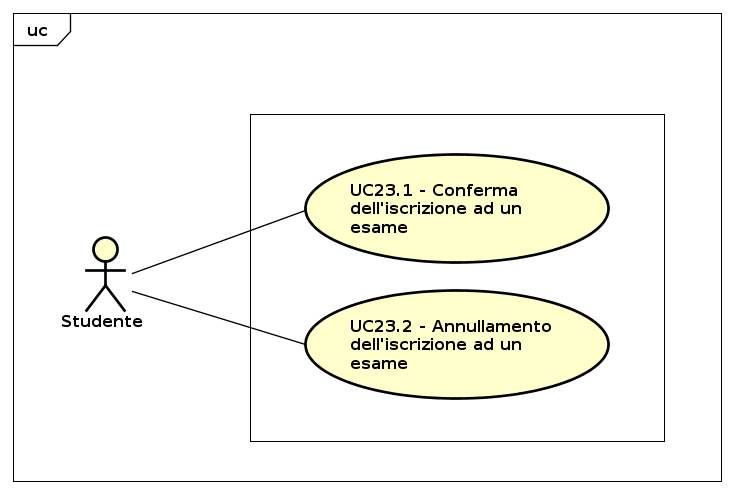
\includegraphics[scale=0.45]{./img/UseCaseDiagram023.png}
%	\caption{Iscrizione ad un esame}\label{}
%\end{figure}
%\begin{itemize}
%	\item \textbf{Attori}: Studente;
%	\item \textbf{Descrizione}: L'attore vedendo la lista degli appelli disponibili si iscrive ad uno di essi;
%	\item \textbf{Precondizione}: Il sistema fa visualizzare la lista degli appelli disponibili per l'attore;
%	\item \textbf{Flusso principale degli eventi}: L'attore si iscrive ad un esame;
%	\begin{itemize}
%		\item Conferma dell'iscrizione ad un esame (UC\ref{Iscrizione ad un esame}.\ref{Conferma dell'iscrizione ad un esame});
%		\item Annullamento dell'iscrizione ad un esame (UC\ref{Iscrizione ad un esame}.\ref{Annullamento dell'iscrizione ad un esame}).
%	\end{itemize}
%	\item \textbf{Postcondizione}: Il sistema fa visualizzare l'appello che l'attore ha selezionato per l'iscrizione.
%\end{itemize}
%
%%{UC6.1}
%\taskOO{Conferma dell'iscrizione ad un esame}
%\subsection{Caso d'uso UC\ref{Iscrizione ad un esame}.\ref{Conferma dell'iscrizione ad un esame}: Conferma dell'iscrizione ad un esame}
%\begin{itemize}
%	\item \textbf{Attori}: Studente;
%	\item \textbf{Descrizione}: L'attore può confermare l'azione di iscrizione ad un esame;
%	\item \textbf{Precondizione}: Il sistema fa visualizzare all'attore l'esame che ha selezionato per l'iscrizione;
%	\item \textbf{Flusso principale degli eventi}: L'attore ha selezionato l'esame a cui iscriversi e può confermare l'azione;
%	\item \textbf{Postcondizione}: Il sistema ha iscritto l'attore a quell'esame.
%\end{itemize}
%
%%{UC6.2}
%\taskOO{Annullamento dell'iscrizione ad un esame}
%\subsection{Caso d'uso UC\ref{Iscrizione ad un esame}.\ref{Annullamento dell'iscrizione ad un esame}: Annullamento dell'iscrizione ad un esame}
%\begin{itemize}
%	\item \textbf{Attori}: Studente;
%	\item \textbf{Descrizione}: L'attore può annullare l'azione di iscrizione ad un esame;
%	\item \textbf{Precondizione}: Il sistema fa visualizzare all'attore l'esame che ha selezionato per l'iscrizione;
%	
%	\item \textbf{Flusso principale degli eventi}: L'attore può annullare l'iscrizione ad un esame dopo averlo selezionato;
%	\item \textbf{Postcondizione}: Il sistema non ha iscritto l'attore a quell'esame in quanto esso ha annullato l'operazione.
%	
%\end{itemize}

%%{UC7}
%\taskO{Eliminazione dell'iscrizione ad un esame}
%\subsection{Caso d'uso UC\ref{Eliminazione dell'iscrizione ad un esame}: Eliminazione dell'iscrizione ad un esame}
%\begin{figure} [H]
%	\centering
%	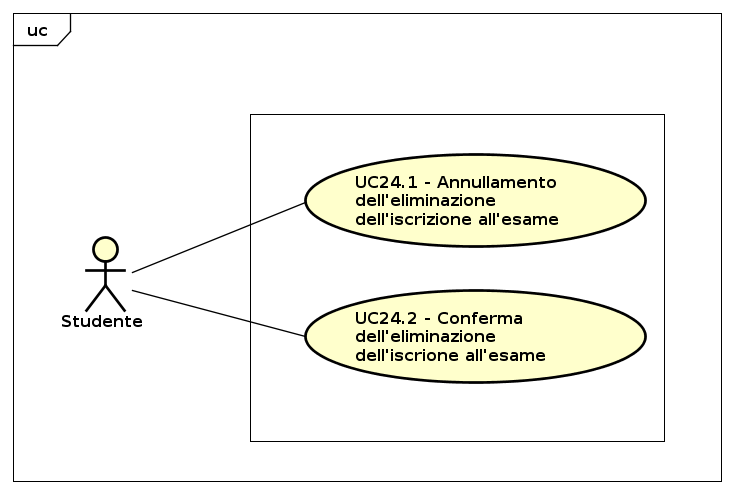
\includegraphics[scale=0.45]{./img/UseCaseDiagram024.png}
%	\caption{Eliminazione dell'iscrizione ad un esame}\label{}
%\end{figure}
%\begin{itemize}
%	\item \textbf{Attori}: Studente;
%	\item \textbf{Descrizione}: L'attore si è precedentemente iscritto ad un esame e può annullarne l'iscrizione;
%	\item \textbf{Precondizione}: Il sistema fa visualizzare all'attore l'esame a cui esso è registrato;
%	\item \textbf{Flusso principale degli eventi}: L'attore vuole eliminare l'iscrizione ad un esame a cui si è precedentemente registrato e può fare due scelte:
%	\begin{itemize}
%		\item Annullamento dell'eliminazione dell'iscrizione ad un esame (UC\ref{Eliminazione dell'iscrizione ad un esame}.\ref{Annullamento dell'eliminazione dell'iscrizione ad un esame});
%		\item Conferma dell'eliminazione dell'iscrizione ad un esame (UC\ref{Eliminazione dell'iscrizione ad un esame}.\ref{Conferma dell'eliminazione dell'iscrizione ad un esame}).
%	\end{itemize}
%	\item \textbf{Postcondizione}: Il sistema disiscrive l'attore a quell'esame.
%\end{itemize}
%
%%{UC7.1}
%\taskOO{Annullamento dell'eliminazione dell'iscrizione ad un esame}
%\subsection{Caso d'uso UC\ref{Eliminazione dell'iscrizione ad un esame}.\ref{Annullamento dell'eliminazione dell'iscrizione ad un esame}: Annullamento dell'eliminazione dell'iscrizione ad un esame}
%\begin{itemize}
%	\item \textbf{Attori}: Studente;
%	\item \textbf{Descrizione}: L'attore sta eliminando l'iscrizione ad un esame ma decide di non farlo;
%	\item \textbf{Precondizione}: Il sistema fa visualizzare all'attore l'esame a cui esso è registrato;
%	
%	\item \textbf{Flusso principale degli eventi}: L'attore che sta eliminando l'iscrizione ad un esame decide di annullare l'operazione;
%	\item \textbf{Postcondizione}: Il sistema non disiscrive più l'attore a quell'esame in quanto esso ha annullato l'operazione.
%	
%\end{itemize}
%
%%{UC7.2}
%\taskOO{Conferma dell'eliminazione dell'iscrizione ad un esame}
%\subsection{Caso d'uso UC\ref{Eliminazione dell'iscrizione ad un esame}.\ref{Conferma dell'eliminazione dell'iscrizione ad un esame}: Conferma dell'eliminazione dell'iscrizione ad un esame}
%\begin{itemize}
%	\item \textbf{Attori}: Studente;
%	\item \textbf{Descrizione}: L'attore che sta eliminando l'iscrizione ad un esame conferma tale scelta;
%	\item \textbf{Precondizione}: Il sistema fa visualizzare all'attore l'esame a cui esso vuole disiscriversi;
%	
%	\item \textbf{Flusso principale degli eventi}: L'attore conferma l'eliminazione di un'iscrizione ad un esame;
%	\item \textbf{Postcondizione}: Il sistema disiscrive l'attore a quell'esame.
%	
%\end{itemize}

%{UC8}
\taskO{Rifiuto del voto di un esame}
\subsection{Caso d'uso UC\ref{Rifiuto del voto di un esame}: Rifiuto del voto di un esame}
\begin{itemize}
	\item \textbf{Attori}: Studente;
	\item \textbf{Descrizione}: L'attore può rifiutare il voto di un esame;
	\item \textbf{Precondizione}: Il sistema fa visualizzare all'attore il voto relativo ad esame che esso ha sostenuto;
	\item \textbf{Flusso principale degli eventi}: L'attore dopo aver visualizzato il voto dell'esame decide di rifiutarne il voto;
	\item \textbf{Postcondizione}: Il sistema non mostra alcun voto relativo a quell'esame in quanto l'attore l'ha rifiutato.
\end{itemize}

%{UC9}
\taskO{Modifica di un esame da parte di un professore}
\subsection{Caso d'uso UC\ref{Modifica di un esame da parte di un professore}: Modifica di un esame da parte di un professore}
\begin{figure} [H]
	\centering
	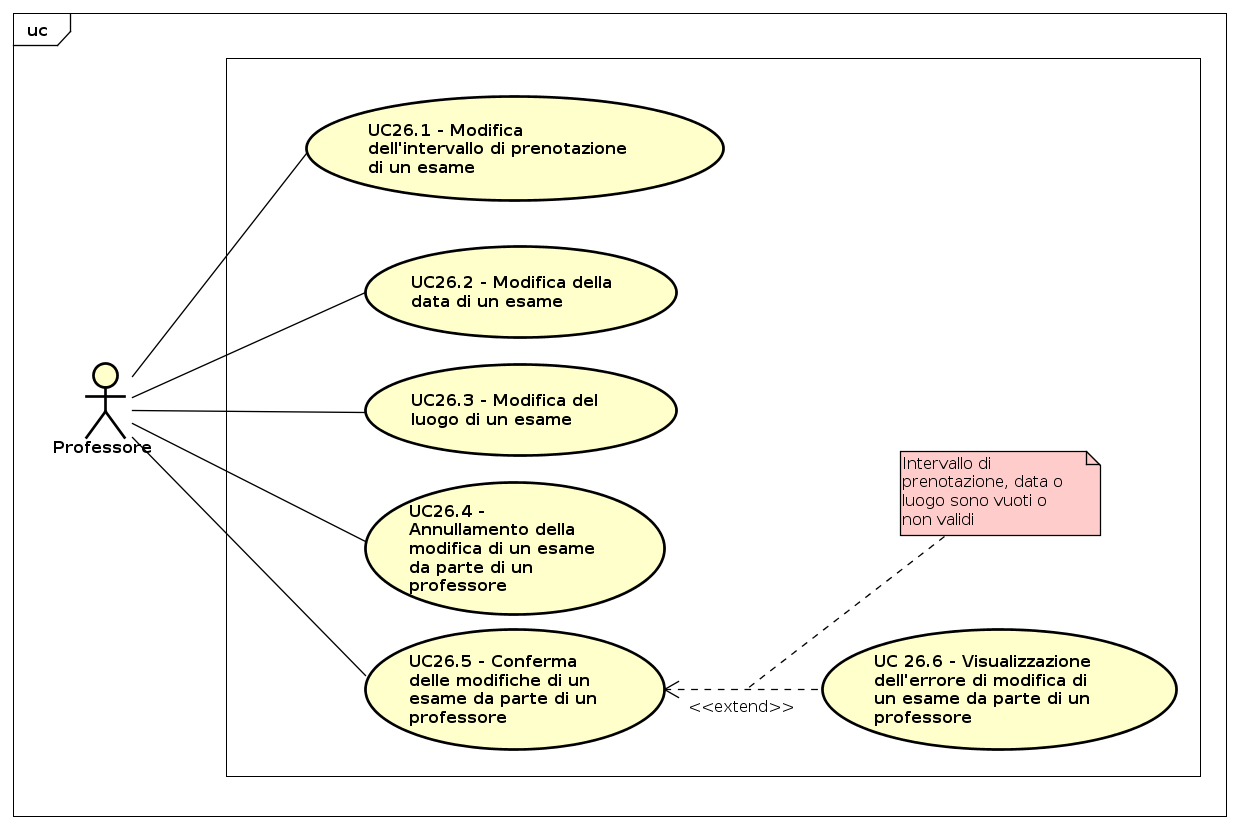
\includegraphics[scale=0.45]{./img/UseCaseDiagram026.png}
	\caption{Modifica di un esame da parte di un professore}\label{}
\end{figure}
\begin{itemize}
	\item \textbf{Attori}: Professore;
	\item \textbf{Descrizione}: L'attore ha accesso alla modifica di alcuni campi dati degli esami a cui sono assegnati;
	\item \textbf{Precondizione}: Il sistema fa visualizzare un esame al professore;
	
	\item \textbf{Flusso principale degli eventi}: L'attore ha possibilità di modifica dei seguenti punti degli esami a cui è assegnato:
	\begin{itemize}
		\item Modifica dell'intervallo di prenotazione di un esame (UC\ref{Modifica di un esame da parte di un professore}.\ref{Modifica dell'intervallo di prenotazione di un esame});
		\item Modifica della data di un esame (UC\ref{Modifica di un esame da parte di un professore}.\ref{Modifica della data di un esame});
		\item Modifica del luogo di un esame (UC\ref{Modifica di un esame da parte di un professore}.\ref{Modifica del luogo di un esame});
		\item Annullamento della modifica di un esame da parte di un professore (UC\ref{Modifica di un esame da parte di un professore}.\ref{Annullamento della modifica di un esame da parte di un professore});
		\item Conferma della modifica di un esame da parte di un professore (UC\ref{Modifica di un esame da parte di un professore}.\ref{Conferma della modifica di un esame da parte di un professore});
		\item Visualizzazione dell'errore di modifica di un esame da parte di un professore ( UC\ref{Modifica di un esame da parte di un professore}.\ref{Visualizzazione dell'errore di modifica di un esame da parte di un professore}).
	\end{itemize}
	\item \textbf{Postcondizione}: Il sistema ha modificato l'esame in quanto il professore ha attuato l'operazione di modifica.
	
\end{itemize}

%{UC9.1}
\taskOO{Modifica dell'intervallo di prenotazione di un esame}
\subsection{Caso d'uso UC\ref{Modifica di un esame da parte di un professore}.\ref{Modifica dell'intervallo di prenotazione di un esame}: Modifica dell'intervallo di prenotazione di un esame}
\begin{itemize}
	\item \textbf{Attori}: Professore;
	\item \textbf{Descrizione}: L'attore modifica l'intervallo temporale per cui uno studente ha la possibilità di iscriversi ad un esame;
	\item \textbf{Precondizione}: Il sistema fa visualizzare un esame al professore;
	
	
	\item \textbf{Flusso principale degli eventi}: L'attore modifica l'intervallo di prenotazione di un esame;
	\item \textbf{Postcondizione}: Il sistema ha modificato l'intervallo di prenotazione per l'esame in quanto il professore ha attuato l'operazione di modifica.
	
\end{itemize}

%{UC9.2}
\taskOO{Modifica della data di un esame}
\subsection{Caso d'uso UC\ref{Modifica di un esame da parte di un professore}.\ref{Modifica della data di un esame}: Modifica della data di un esame}
\begin{itemize}
	\item \textbf{Attori}: Professore;
	\item \textbf{Descrizione}: L'attore ha la possibilità di modificare la data di un esame;
	\item \textbf{Precondizione}: Il sistema fa visualizzare un esame al professore;
	
	\item \textbf{Flusso principale degli eventi}: L'attore modifica la data di un esame;
	\item \textbf{Postcondizione}: Il sistema ha modificato l'intervallo di prenotazione per l'esame in quanto il professore ha attuato l'operazione di modifica.
	
\end{itemize}

%{UC9.3}
\taskOO{Modifica del luogo di un esame}
\subsection{Caso d'uso UC\ref{Modifica di un esame da parte di un professore}.\ref{Modifica del luogo di un esame}: Modifica del luogo di un esame}
\begin{itemize}
	\item \textbf{Attori}: Professore;
	\item \textbf{Descrizione}: L'attore ha la possibilità di modificare il luogo degli esami a cui è assegnato;
	\item \textbf{Precondizione}: Il sistema fa visualizzare un esame al professore;
	
	\item \textbf{Flusso principale degli eventi}: L'attore modifica il luogo di un esame;
	\item \textbf{Postcondizione}: Il sistema ha modificato il luogo dell'esame in quanto il professore ha attuato l'operazione di modifica.
	
\end{itemize}

%{UC9.4}
\taskOO{Annullamento della modifica di un esame da parte di un professore}
\subsection{Caso d'uso UC\ref{Modifica di un esame da parte di un professore}.\ref{Annullamento della modifica di un esame da parte di un professore}: Annullamento della modifica di un esame da parte di un professore}
\begin{itemize}
	\item \textbf{Attori}: Professore;
	\item \textbf{Descrizione}: L'attore che sta modificando un esame decide di annullare l'operazione;
	\item \textbf{Precondizione}: Il sistema fa visualizzare al professore la pagina relativa alla modifica di un esame;
	
	\item \textbf{Flusso principale degli eventi}: L'attore annulla le modifiche che sta compiendo;
	\item \textbf{Postcondizione}: Il sistema non modifica più un esame in quanto il professore ha annullato l'operazione.
	
\end{itemize}

%{UC9.5}
\taskOO{Conferma della modifica di un esame da parte di un professore}
\subsection{Caso d'uso UC\ref{Modifica di un esame da parte di un professore}.\ref{Conferma della modifica di un esame da parte di un professore}: Conferma della modifica di un esame da parte di un professore}
\begin{itemize}
	\item \textbf{Attori}: Professore;
	\item \textbf{Descrizione}: L'attore che sta modificando un esame decide di confermare le modifiche;
	\item \textbf{Precondizione}: Il sistema fa visualizzare al professore la pagina relativa alla modifica di un esame;
	
	\item \textbf{Flusso principale degli eventi}: L'attore conferma le modifiche fatte all'esame;
	\item \textbf{Postcondizione}: Il sistema modifica un esame in quanto il professore ha confermato l'operazione;
	
	\item \textbf{Estensioni}:
	\begin{itemize}
		\item Visualizzazione dell'errore di modifica di un esame da parte di un professore ( UC\ref{Modifica di un esame da parte di un professore}.\ref{Visualizzazione dell'errore di modifica di un esame da parte di un professore}).
	\end{itemize}
\end{itemize}

%{UC9.6}
\taskOO{Visualizzazione dell'errore di modifica di un esame da parte di un professore}
\subsection{Caso d'uso UC\ref{Modifica di un esame da parte di un professore}.\ref{Visualizzazione dell'errore di modifica di un esame da parte di un professore}: Visualizzazione dell'errore di modifica di un esame da parte di un professore}
\begin{itemize}
	\item \textbf{Attori}: Professore;
	\item \textbf{Descrizione}: Il sistema visualizza un errore riguardante l'errata modifica dei campi dati di un esame;
	\item \textbf{Precondizione}: Il sistema ha ricevuto campi dati errati o vuoti da parte di un professore;
	
	\item \textbf{Flusso principale degli eventi}: L'attore, modificando in maniera errata i campi dell'esame, può visualizzare uno dei seguenti errori: \begin{itemize}
		\item Intervallo di prenotazione per l'esame non valido o lasciato vuoto;
		\item Data dell'esame non valida o lasciato vuoto;
		\item Luogo d'esame non valido o lasciato vuoto.
	\end{itemize}
	\item \textbf{Postcondizione}: Il sistema fa visualizzare al professore un messaggio d'errore relativo all'operazione di modifica di un esame
	
\end{itemize}


%UC10
\taskO{Inserimento di un voto}
\subsection{Caso d'uso UC\ref{Inserimento di un voto}: Inserimento di un voto }
\begin{figure} [H]
	\centering
	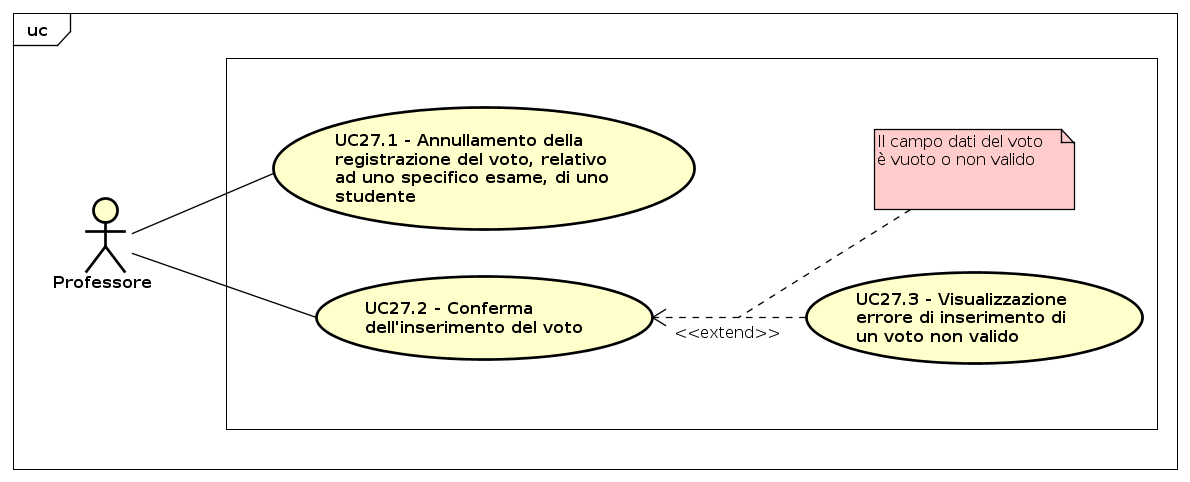
\includegraphics[scale=0.45]{./img/UseCaseDiagram027.png}
	\caption{Inserimento di un voto }\label{}
\end{figure}
\begin{itemize}
	\item \textbf{Attori}: Professore;
	\item \textbf{Descrizione}: L'attore visualizza la lista degli studenti iscritti all'esame e assegna una votazione;
	\item \textbf{Precondizione}: Il sistema fa visualizzare all'attore la lista degli studenti iscritti all'esame;
	\item \textbf{Flusso principale degli eventi}: L'attore inserendo un voto ad uno studente si trova davanti ai seguenti scenari;
	\begin{itemize}
		\item Annullamento della registrazione del voto, relativo ad uno specifico esame, di uno studente (UC\ref{Inserimento di un voto}.\ref{Annullamento della registrazione del voto, relativo ad uno specifico esame, di uno studente});
		\item Conferma dell'inserimento di un voto (UC\ref{Inserimento di un voto}.\ref{Conferma dell'inserimento di un voto});
		\item Visualizzazione dell'errore di inserimento di un voto non valido (UC\ref{Inserimento di un voto}.\ref{Visualizzazione dell'errore di inserimento di un voto non valido}).
	\end{itemize}
	\item \textbf{Postcondizione}: Il sistema fa visualizzare il campo, che può essere stato compilato, relativo al voto di uno studente per un esame.
\end{itemize}

%{UC10.1}
\taskOO{Annullamento della registrazione del voto, relativo ad uno specifico esame, di uno studente}
\subsection{Caso d'uso UC\ref{Inserimento di un voto}.\ref{Annullamento della registrazione del voto, relativo ad uno specifico esame, di uno studente}: Annullamento della registrazione del voto, relativo ad uno specifico esame, di uno studente}
\begin{itemize}
	\item \textbf{Attori}: Professore;
	\item \textbf{Descrizione}: L'attore sta inserendo il voto ad uno studente e decide di annullare l'operazione;
	\item \textbf{Precondizione}: Il sistema fa visualizzare all'attore la lista degli studenti iscritti all'esame;
	
	\item \textbf{Flusso principale degli eventi}: L'attore che sta inserendo un voto può decidere di annullare l'operazione;
	\item \textbf{Postcondizione}: Il sistema non inserisce più il voto allo studente in quanto l'attore ha annullato l'operazione.
	
\end{itemize}

%{UC10.2}
\taskOO{Conferma dell'inserimento di un voto}
\subsection{Caso d'uso UC\ref{Inserimento di un voto}.\ref{Conferma dell'inserimento di un voto}: Conferma dell'inserimento di un voto}
\begin{itemize}
	\item \textbf{Attori}: Professore;
	\item \textbf{Descrizione}: L'attore dopo aver immesso il voto dello studete decide di confermarlo;
	\item \textbf{Precondizione}: Il sistema fa visualizzare il campo, che può essere stato compilato, relativo al voto di uno studente per un esame;
	\item \textbf{Flusso principale degli eventi}: L'attore che inserisce il voto allo studente può confermarlo;
	\item \textbf{Postcondizione}: Il sistema inserisce il voto allo studente in quanto l'attore ha confermato l'operazione.
	\item \textbf{Estensioni}:
	\begin{itemize}
		\item Visualizzazione dell'errore di inserimento di un voto non valido (UC\ref{Inserimento di un voto}.\ref{Visualizzazione dell'errore di inserimento di un voto non valido}).
	\end{itemize}
\end{itemize}

%{UC10.3}
\taskOO{Visualizzazione dell'errore di inserimento di un voto non valido}
\subsection{Caso d'uso UC\ref{Inserimento di un voto}.\ref{Visualizzazione dell'errore di inserimento di un voto non valido}: Visualizzazione dell'errore di inserimento di un voto non valido}
\begin{itemize}
	\item \textbf{Attori}: Professore;
	\item \textbf{Descrizione}: Il sistema visualizza un messaggio di errore causato dall'immissione di un voto non conforme;
	\item \textbf{Precondizione}: Il sistema ha ricevuto un voto non valido;
	
	\item \textbf{Flusso principale degli eventi}: L'attore, che sbaglia ad inserire un voto, visualizza un messaggio d'errore relativo ad esso;
	\item \textbf{Postcondizione}: Il sistema fa visualizzare un messaggio d'errore riguardante il tentativo di inserire un voto non valido.
\end{itemize}




%{UC11}
\taskO{Inserimento di un utente nel sistema}
\subsection{Caso d'uso UC\ref{Inserimento di un utente nel sistema}: Inserimento di un utente nel sistema}
\begin{figure} [H]
	\centering
	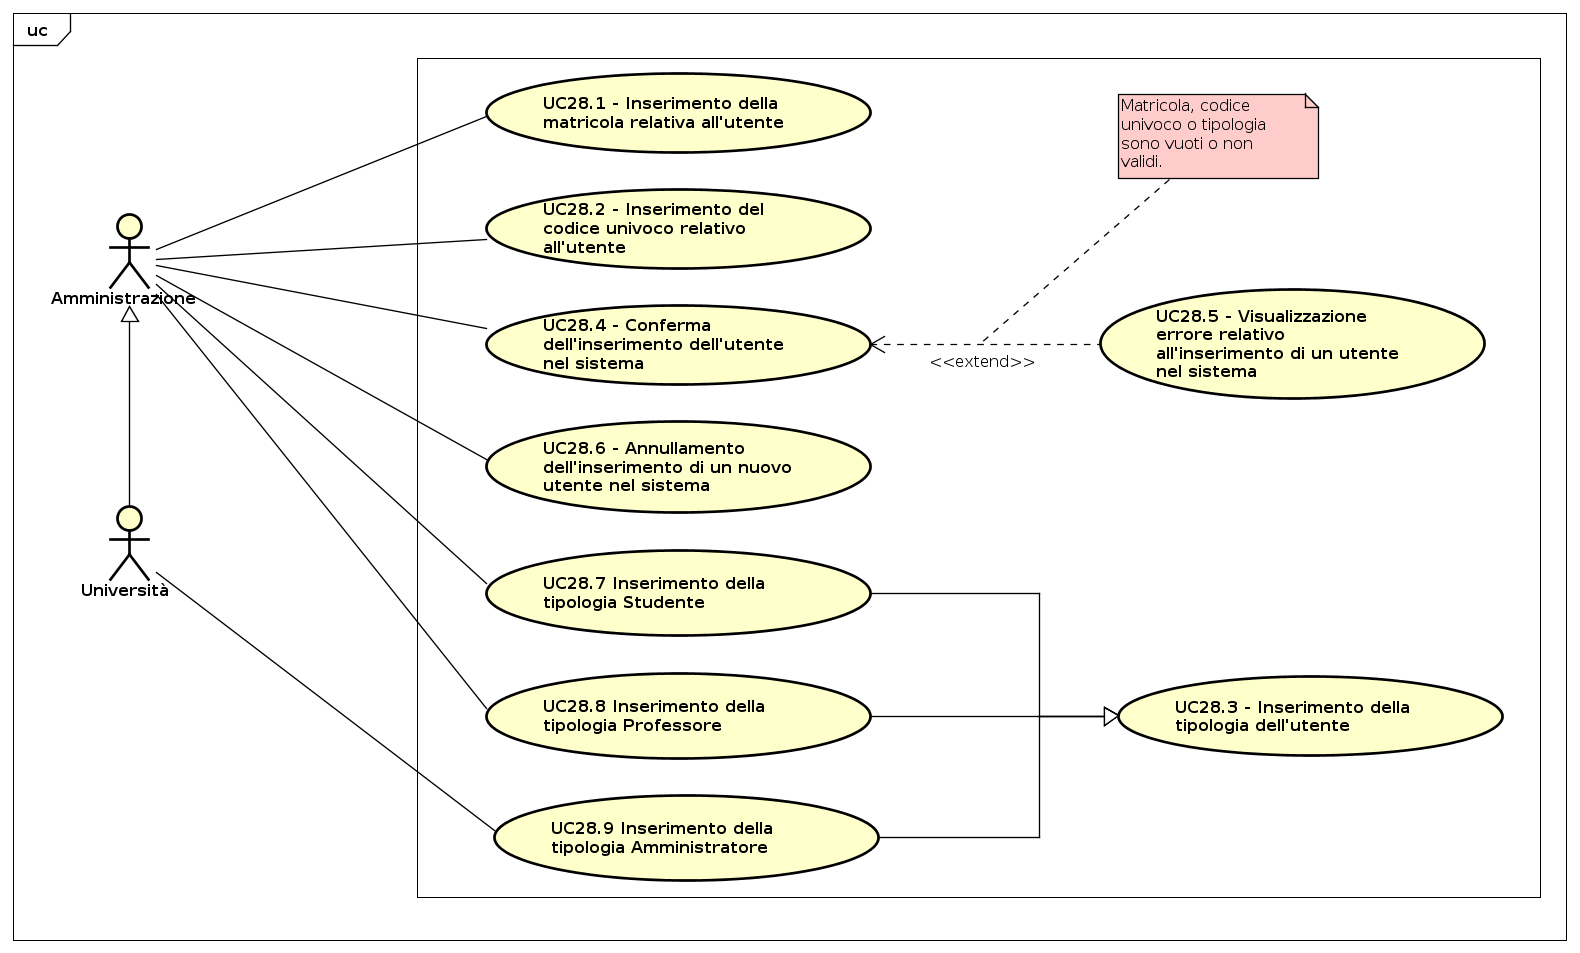
\includegraphics[scale=0.45]{./img/UseCaseDiagram028.png}
	\caption{Inserimento di un utente nel sistema}\label{}
\end{figure}
\begin{itemize}
	\item \textbf{Attori}: Amministratore, Università;
	\item \textbf{Descrizione}: L'attore può inserire un nuovo utente nel sistema;
	\item \textbf{Precondizione}: Il sistema è pronto per inserire un nuovo utente;
	\item \textbf{Flusso principale degli eventi}: L'attore può inserire un nuovo utente nel sistema, che non sia già presente in esso, seguendo i seguenti passi:
	\begin{itemize}
		\item Inserimento della matricola relativa ad un utente (UC\ref{Inserimento di un utente nel sistema}.\ref{Inserimento della matricola relativa ad un utente});
		\item Inserimento del codice univoco relativo ad un utente (UC\ref{Inserimento di un utente nel sistema}.\ref{Inserimento del codice univoco relativo ad un utente});
		\item Inserimento della tipologia di un utente (UC\ref{Inserimento di un utente nel sistema}.\ref{Inserimento della tipologia di un utente});
		\item Conferma dell'inserimento di un utente nel sistema (UC\ref{Inserimento di un utente nel sistema}.\ref{Conferma dell'inserimento di un utente nel sistema});
		\item Visualizzazione dell'errore relativo all'inserimento di un utente nel sistema (UC\ref{Inserimento di un utente nel sistema}.\ref{Visualizzazione dell'errore relativo all'inserimento di un utente nel sistema});
		\item Annullamento dell'inserimento di un nuovo utente nel sistema (UC\ref{Inserimento di un utente nel sistema}.\ref{Annullamento dell'inserimento di un nuovo utente nel sistema});
		\item Inserimento della tipologia Studente (UC11.7);
		\item Inserimento della tipologia Professore (UC11.8);
		\item Inserimento della tipologia Amministratore (UC11.9).
	\end{itemize}
	\item \textbf{Postcondizione}: Il sistema può aver compilato dei campi relativi all'inserimento di un utente nel sistema.
	
\end{itemize}

%{UC11.1}
\taskOO{Inserimento della matricola relativa ad un utente}
\subsection{Caso d'uso UC\ref{Inserimento di un utente nel sistema}.\ref{Inserimento della matricola relativa ad un utente}: Inserimento della matricola relativa ad un utente}
\begin{itemize}
	\item \textbf{Attori}: Amministratore, Università;
	\item \textbf{Descrizione}: L'attore può inserire la matricola relativa all'utente;
	\item \textbf{Precondizione}: Il sistema fa visualizzare il campo della matricola relativa all'utente;
	\item \textbf{Flusso principale degli eventi}: L'attore può inserire la matricola dell'utente durante il suo inserimento nel sistema;
	\item \textbf{Postcondizione}: È stata inserita la matricola relativa all'utente nel campo opportuno.
\end{itemize}

%{UC11.2}
\taskOO{Inserimento del codice univoco relativo ad un utente}
\subsection{Caso d'uso UC\ref{Inserimento di un utente nel sistema}.\ref{Inserimento del codice univoco relativo ad un utente}: Inserimento del codice univoco relativo ad un utente}
\begin{itemize}
	\item \textbf{Attori}: Amministratore, Università;
	\item \textbf{Descrizione}: L'attore può inserire il codice univoco relativo all'utente;
	\item \textbf{Precondizione}: Il sistema fa visualizzare il campo del codice univoco relativo all'utente;
	
	\item \textbf{Flusso principale degli eventi}: L'attore può inserire il codice univoco dell'utente durante il suo inserimento nel sistema;
	\item \textbf{Postcondizione}: È stato inserito il codice univoco relativo all'utente nel campo opportuno.
	
\end{itemize}

%{UC11.3}
\taskOO{Inserimento della tipologia di un utente}
\subsection{Caso d'uso UC\ref{Inserimento di un utente nel sistema}.\ref{Inserimento della tipologia di un utente}: Inserimento della tipologia di un utente }
\begin{itemize}
	\item \textbf{Attori}: Amministratore, Università;
	\item \textbf{Descrizione}: L'attore può inserire la tipologia relativa all'utente;
	\item \textbf{Precondizione}: Il sistema fa visualizzare il campo della tipologia di un utente;
	
	\item \textbf{Flusso principale degli eventi}: L'attore può inserire la tipologia dell'utente;
	\item \textbf{Postcondizione}: È stata inserita la tipologia di un utente nel campo opportuno;
	\item \textbf{Generalizzazioni}:
	\begin{itemize}
		\item Inserimento della tipologia Studente (UC\ref{Inserimento di un utente nel sistema}.\ref{Inserimento della tipologia Studente}); 
		\item Inserimento della tipologia Professore (UC\ref{Inserimento di un utente nel sistema}.\ref{Inserimento della tipologia Professore});
		\item Inserimento della tipologia Amministratore (UC\ref{Inserimento di un utente nel sistema}.\ref{Inserimento della tipologia Amministratore}).
	\end{itemize}
	
\end{itemize}

%{UC11.4}
\taskOO{Conferma dell'inserimento di un utente nel sistema}
\subsection{Caso d'uso UC\ref{Inserimento di un utente nel sistema}.\ref{Conferma dell'inserimento di un utente nel sistema}: Conferma dell'inserimento di un utente nel sistema}
\begin{itemize}
	\item \textbf{Attori}: Amministratore, Università;
	\item \textbf{Descrizione}: L'attore può confermare l'inserimento nel sistema;
	\item \textbf{Precondizione}: Il sistema fa visualizzare il campo, che può essere stato compilato, relativo all'inserimento di un utente nel sistema;
	\item \textbf{Flusso principale degli eventi}: L'attore può confermare l'inserimento dell'utente nel sistema;
	\item \textbf{Postcondizione}: Il sistema inserisce un nuovo utente in quanto l'attore ha confermato l'operazione.
	
	\item \textbf{Estensioni}:
	\begin{itemize}
		\item Visualizzazione dell'errore relativo all'inserimento di un utente nel sistema (UC\ref{Inserimento di un utente nel sistema}.\ref{Visualizzazione dell'errore relativo all'inserimento di un utente nel sistema}).
	\end{itemize}
\end{itemize}

%{UC11.5}
\taskOO{Visualizzazione dell'errore relativo all'inserimento di un utente nel sistema}
\subsection{Caso d'uso UC\ref{Inserimento di un utente nel sistema}.\ref{Visualizzazione dell'errore relativo all'inserimento di un utente nel sistema}: Visualizzazione dell'errore relativo all'inserimento di un utente nel sistema}
\begin{itemize}
	\item \textbf{Attori}: Amministratore, Università;
	\item \textbf{Descrizione}: L'attore aggiunge i dettagli relativi all'inserimento di un utente nel sistema senza rispettarne la validazione;
	\item \textbf{Precondizione}: Il sistema ha ricevuto campi dati errati o vuoti;
	
	
	\item \textbf{Flusso principale degli eventi}: L'attore, impostando in maniera errata i campi dell'utente, può visualizzare uno dei seguenti errori:
	\begin{itemize}
		\item Matricola non valida oppure lasciata vuota;
		\item Codice univoco non valido oppure lasciato vuoto.
	\end{itemize}
	\item \textbf{Postcondizione}: Il sistema fa visualizzare un messaggio d'errore riguardante il tentativo di inserire un nuovo utente.
	
\end{itemize}

%{UC11.6}
\taskOO{Annullamento dell'inserimento di un nuovo utente nel sistema}
\subsection{Caso d'uso UC\ref{Inserimento di un utente nel sistema}.\ref{Annullamento dell'inserimento di un nuovo utente nel sistema}: Annullamento dell'inserimento di un nuovo utente nel sistema}
\begin{itemize}
	\item \textbf{Attori}: Amministratore, Università;
	\item \textbf{Descrizione}: L'attore non inserisce più un nuovo utente nel sistema;
	\item \textbf{Precondizione}: l sistema fa visualizzare la pagina relativa all'inserimento di un nuovo utente nel sistema;
	
	\item \textbf{Flusso principale degli eventi}: L'attore non inserisce più un nuovo utente nel sistema e quindi annulla l'operazione;
	\item \textbf{Postcondizione}: Il sistema non aggiunge più un nuovo utente in quanto l'attore ha annullato l'operazione.
	
\end{itemize}

%{UC11.7}
\taskOO{Inserimento della tipologia Studente}
\subsection{Caso d'uso UC\ref{Inserimento di un utente nel sistema}.\ref{Inserimento della tipologia Studente}: Inserimento della tipologia Studente}
\begin{itemize}
	\item \textbf{Attori}: Amministratore, Università;
	\item \textbf{Descrizione}: L'attore ha scelto studente come tipologia di utente; 
	\item \textbf{Precondizione}: Il sistema permette la scelta della tipologia di utente;
	\item \textbf{Flusso principale degli eventi}: L'attore può scegliere quale tipologia di utente inserire;
	\item \textbf{Postcondizione}: Come tipologia di utente è stato scelto lo studente;
\end{itemize}

%{UC11.8}
\taskOO{Inserimento della tipologia Professore}
\subsection{Caso d'uso UC\ref{Inserimento di un utente nel sistema}.\ref{Inserimento della tipologia Professore}: Inserimento della tipologia Professore}
\begin{itemize}
	\item \textbf{Attori}: Amministratore, Università;
	\item \textbf{Descrizione}: L'attore ha scelto professore come tipologia di utente; 
	\item \textbf{Precondizione}: Il sistema permette la scelta della tipologia di utente;
	\item \textbf{Flusso principale degli eventi}: L'attore può scegliere quale tipologia di utente inserire;
	\item \textbf{Postcondizione}: Come tipologia di utente è stato scelto il professore;
\end{itemize}

%{UC11.9}
\taskOO{Inserimento della tipologia Amministratore}
\subsection{Caso d'uso UC\ref{Inserimento di un utente nel sistema}.\ref{Inserimento della tipologia Amministratore}: Inserimento della tipologia Amministratore}
\begin{itemize}
	\item \textbf{Attori}: Università;
	\item \textbf{Descrizione}: L'attore ha scelto amministratore come tipologia di utente; 
	\item \textbf{Precondizione}: Il sistema permette la scelta della tipologia di utente;
	\item \textbf{Flusso principale degli eventi}: L'attore può scegliere quale tipologia di utente inserire;
	\item \textbf{Postcondizione}: Come tipologia di utente è stato scelto l'amministratore;
\end{itemize}



%UC12
\taskO{Rimozione di un utente dal sistema}
\subsection{Caso d'uso UC\ref{Rimozione di un utente dal sistema}: Rimozione di un utente dal sistema}
\begin{figure} [H]
	\centering
	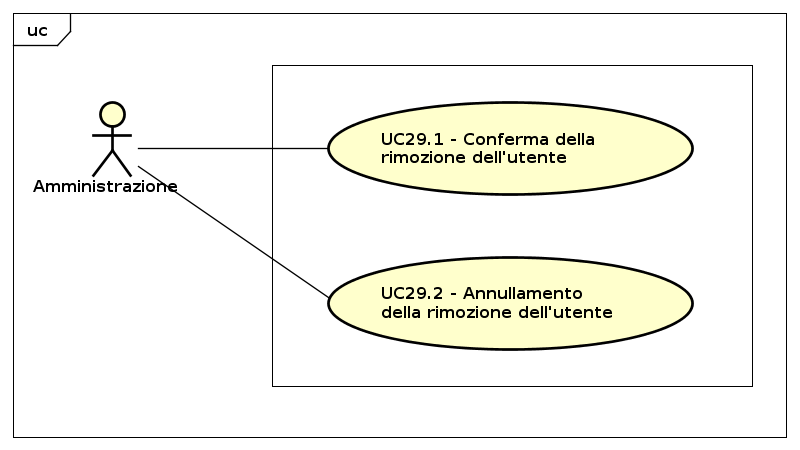
\includegraphics[scale=0.45]{./img/UseCaseDiagram029.png}
	\caption{Rimozione di un utente dal sistema}\label{}
\end{figure}
\begin{itemize}
	\item \textbf{Attori}: Amministratore, Università;
	\item \textbf{Descrizione}: L'attore può rimuovere un utente, cancellandone tutti i dati ad esso associati nonché rimuovendone l'accesso al sistema;
	\item \textbf{Precondizione}: Il sistema riconosce come registrato l'utente che l'attore ha selezionato;
	\item \textbf{Flusso principale degli eventi}: L'attore, volendo rimuovere completamente un utente dal sistema, si troverà davanti alle seguenti scelte:
	\begin{itemize}
		\item Conferma della rimozione di un utente dal sistema (UC\ref{Rimozione di un utente dal sistema}.\ref{Conferma della rimozione di un utente dal sistema});
		\item Annullamento della rimozione di un utente dal sistema (UC\ref{Rimozione di un utente dal sistema}.\ref{Annullamento della rimozione di un utente dal sistema}).
	\end{itemize}
	\item \textbf{Postcondizione}: Il sistema fa visualizzare all'attore l'utente che ha selezionato per rimuoverlo dal sistema;
\end{itemize}

%{UC12.1}
\taskOO{Conferma della rimozione di un utente dal sistema}
\subsection{Caso d'uso UC\ref{Rimozione di un utente dal sistema}.\ref{Conferma della rimozione di un utente dal sistema}: Conferma della rimozione di un utente dal sistema}
\begin{itemize}
	\item \textbf{Attori}: Amministratore, Università;
	\item \textbf{Descrizione}: L'attore può confermare la rimozione di un utente dal sistema;
	\item \textbf{Precondizione}: Il sistema fa visualizzare all'attore l'utente che ha selezionato per rimuoverlo dal sistema;
	\item \textbf{Flusso principale degli eventi}: L'attore può confermare la rimozione di un utente dal sistema;
	\item \textbf{Postcondizione}: Il sistema ha cancellato la registrazione dell'utente nel sistema e tutti i suoi dati sono stati cancellati.
\end{itemize}

%{UC12.2}
\taskOO{Annullamento della rimozione di un utente dal sistema}
\subsection{Caso d'uso UC\ref{Rimozione di un utente dal sistema}.\ref{Annullamento della rimozione di un utente dal sistema}: Annullamento della rimozione di un utente dal sistema}
\begin{itemize}
	\item \textbf{Attori}: Amministratore, Università;
	\item \textbf{Descrizione}: L'attore può annullare la rimozione di un utente dal sistema;
	\item \textbf{Precondizione}: Il sistema fa visualizzare all'attore l'utente che ha selezionato per rimuoverlo dal sistema;
	
	\item \textbf{Flusso principale degli eventi}: L'attore può annullare l'azione di rimozione di un utente dal sistema;
	\item \textbf{Postcondizione}: Il sistema non cancella più la registrazione dell'utente nel sistema in quanto l'attore ha annullato l'operazione.
	
\end{itemize}


%UC14
\taskO{Visualizzazione del libretto}
\subsection{Caso d'uso UC\ref{Visualizzazione del libretto}: Visualizzazione del libretto}
\begin{itemize}
	\item \textbf{Attori}: Studente;
	\item \textbf{Descrizione}: L'attore può visualizzare la lista di tutti gli esami ha sostenuto o dovrà sostenere;
	\item \textbf{Precondizione}: Il sistema ha registrati uno o più studenti;
	\item \textbf{Flusso principale degli eventi}: L'attore può visualizzare il suo libretto;
	\item \textbf{Postcondizione}: Il sistema fa visualizzare all'attore la lista degli esami sostenuti o che esso dovrà sostenere, che è il libretto.
\end{itemize}

%UC15
\taskO{Visualizzazione degli esami associati}
\subsection{Caso d'uso UC\ref{Visualizzazione degli esami associati}: Visualizzazione degli esami associati}
\begin{itemize}
	\item \textbf{Attori}: Professore;
	\item \textbf{Descrizione}: L'attore può visualizzare la lista di tutti gli esami ad esso associati;
	\item \textbf{Precondizione}: Il sistema ha registrati uno o più professori;
	\item \textbf{Flusso principale degli eventi}: L'attore può visualizzare tutti gli esami che gli sono associati;
	\item \textbf{Postcondizione}: Il sistema fa visualizzare tutti gli esami associati all'attore.
\end{itemize}

%UC16
\taskO{Visualizzazione degli studenti iscritti ad un esame associato}
\subsection{Caso d'uso UC\ref{Visualizzazione degli studenti iscritti ad un esame associato}: Visualizzazione degli studenti iscritti ad un esame associato}
\begin{itemize}
	\item \textbf{Attori}: Professore;
	\item \textbf{Descrizione}: L'attore può visualizzare tutti gli studenti che sono iscritti ad un esame a lui associato;
	\item \textbf{Precondizione}: Il sistema ha registrati uno o più professori e uno o più esami ad essi associati;
	\item \textbf{Flusso principale degli eventi}: L'attore può visualizzare la lista degli studenti che si sono iscritti ad un esame a lui associato;
	\item \textbf{Postcondizione}: Il sistema fa visualizzare una lista di studenti che sono iscritti ad un'esame associato all'attore.
\end{itemize}

\taskO{Visualizzazione degli esami con iscrizione effettuata}
\subsection{Caso d'uso UC\ref{Visualizzazione degli esami con iscrizione effettuata}: Visualizzazione degli esami con iscrizione effettuata}
\begin{itemize}
	\item \textbf{Attori}: Studente;
	\item \textbf{Descrizione}: L'attore può visualizzare tutti gli esami a cui ha effettuato l'iscrizione;
	\item \textbf{Precondizione}: Il sistema ha registrati uno o più studenti e zero o più esami ad essi associati;
	\item \textbf{Flusso principale degli eventi}: L'attore può visualizzare la lista degli esami ha cui ha effettuato l'iscrizione;
	\item \textbf{Postcondizione}: Il sistema fa visualizzare una lista di esami a cui lo studente ha effettuato l'iscrizione.
\end{itemize}